%-----------------
% verso e anverso:
%-----------------
%\documentclass[10pt,twoside,openany,a4paper,portuguese]{abntex2}	
\documentclass[
	% -- opções da classe memoir --
	12pt,				% tamanho da fonte
	openany,			% capítulos começam em qualquer página
	%openright,            capítulos começam em pág ímpar (insere página vazia caso preciso)
	%twoside,			% para impressão em verso e anverso. Oposto a oneside	
	oneside,	
	a4paper,			% tamanho do papel. 
	% -- opções da classe abntex2 --
	%chapter=TITLE,		% títulos de capítulos convertidos em letras maiúsculas
	%section=TITLE,		% títulos de seções convertidos em letras maiúsculas
	%subsection=TITLE,	% títulos de subseções convertidos em letras maiúsculas
	%subsubsection=TITLE,% títulos de subsubseções convertidos em letras maiúsculas
	% -- opções do pacote babel --
	brazil,				% o último idioma é o principal do documento
	]{unimontes-ppgmsc-abntex2}

% -------
% PACOTES
% -------

% --------------------
% Pacotes fundamentais 
% --------------------

\usepackage{cmap}				% Mapear caracteres especiais no PDF
\usepackage{lmodern}			% Usa a fonte Latin Modern
\usepackage[utf8]{inputenc}		% Codificacao do documento (conversão automática dos acentos)
\usepackage[T1]{fontenc}		% Selecao de codigos de fonte.
\usepackage{tikz,fullpage}
\usepackage{indentfirst}		% Indenta o primeiro parágrafo de cada seção.
\usepackage{color}				% Controle das cores
\usepackage{graphicx}			% Inclusão de gráficos
\usepackage{pict2e}				% Pacotes graficos para figuras usando comandos de LaTeX
\usepackage{xcolor}
\usepackage{listings}           % Inclusão de arquivos de código de programação
\usepackage{showexpl}           % exibe codigos de figuras
\usepackage{verbatim}           % incluir arquivos não processados pelo Latex
\usepackage{colortbl}
\usepackage{placeins}
\usepackage{amsthm} 			% amsthm -> teorema de demonstracao
\usepackage{amsmath} 			% amsmath -> recursos avancados de matematica
\usepackage{amssymb} 			% amssymb -> symbolos e fontes adicionais (ele inclui amsfonts)
\usepackage{enumerate}			% para configurar a lista enumerada
\usepackage{longtable}			% tabela longa que quebra entre páginas
\usepackage{hhline}				% linhas duplas na tabela
\usepackage{diagbox} % tabela diagonal
\usepackage{mathtools}
\usepackage{float}
%\usepackage[top=3cm, bottom=2cm, left=3cm, right=2cm]{geometry}

%\renewcommand{\pretextual}{\pagenumbering{arabic}}

%% Customiza comando \pretextual
\renewcommand{\pretextual}{
  \pagenumbering{roman} %%% ou \pagenumbering{Roman}
  \pagestyle{plain}
}

% ---
% Ajusta a marca \textual para que a numeração volte a ser arábica
% nos elementos textuais
\let\oldtextual\textual        % copia o comando \textual anterior para \oldtextual
\renewcommand{\textual}{%
  \oldtextual%
  \pagenumbering{arabic} % volta à numeração arábica
  \setcounter{page}{10}
}
% ---

% -------------------
% Pacotes de citações
% -------------------

%\usepackage[brazilian,hyperpageref]{backref}	 % Paginas com as citações na bibl
\usepackage[alf, abnt-url-package=url,]{abntex2cite}	% Citações padrão ABNT

%-----------------------------
% Declarações do algoritmo em Português 
%-----------------------------

\usepackage[Algoritmo]{algorithm}
\usepackage{algpseudocode}

\algrenewcommand\algorithmicend{\textbf{fim}}
\algrenewcommand\algorithmicdo{\textbf{faça}}
\algrenewcommand\algorithmicwhile{\textbf{enquanto}}
\algrenewcommand\algorithmicfor{\textbf{para}}
\algrenewcommand\algorithmicif{\textbf{se}}
\algrenewcommand\algorithmicthen{\textbf{então}}
\algrenewcommand\algorithmicelse{\textbf{senão}}
\algrenewcommand\algorithmicreturn{\textbf{devolve}}
\algrenewcommand\algorithmicfunction{\textbf{função}}
\algnewcommand\algorithmicto{\textbf{até}}

\algrenewtext{EndWhile}{\algorithmicend\ \algorithmicwhile}
\algrenewtext{EndFor}{\algorithmicend\ \algorithmicfor}
\algrenewtext{EndIf}{\algorithmicend\ \algorithmicif}
\algrenewtext{EndFunction}{\algorithmicend\ \algorithmicfunction}

\algnewcommand\algorithmicinput{\textbf{Entrada:}}
\algnewcommand\INPUT{\item[\algorithmicinput]}
\algnewcommand\algorithmicoutput{\textbf{Saída:}}
\algnewcommand\OUTPUT{\item[\algorithmicinput]}

\DeclarePairedDelimiter{\ceil}{\lceil}{\rceil}

\renewcommand{\arraystretch}{1.8} % espaçamento célula da tabela


% ------------------------ 
% CONFIGURAÇÕES DE PACOTES
% ------------------------

% -------------------------------
% Configurações do pacote backref
% Usado sem a opção hyperpageref de backref
%\renewcommand{\backrefpagesname}{Citado na(s) página(s):~}
% Texto padrão antes do número das páginas
%\renewcommand{\backref}{}
% Define os textos da citação
%\renewcommand*{\backrefalt}[4]{
%	\ifcase #1 %
%		Nenhuma citação no texto.%
%	\or
%		Citado na página #2.%
%	\else
%		Citado #1 vezes nas páginas #2.%
%	\fi}%


\headheight 1.4 cm
%\footheight 0.5cm
% ---

%\setlist[itemize,enumerate]{leftmargin=0.7in}


% -----------------------------------------------
% Informações de dados para CAPA e FOLHA DE ROSTO
% -----------------------------------------------
\titulo{Proposta de um Algoritmo Baseado em Particle Swarm Optimization (PSO) para Classificação de Dados}
\autor{Thiago Silva Prates}
\local{Montes Claros - MG}
\data{Abril de 2017}
\instituicao{UNIVERSIDADE ESTADUAL DE MONTES CLAROS \par Centro de Ciências Exatas e Tecnológicas \par Programa de Pós-Graduação Modelagem Computacional e Sistemas} 
\tipotrabalho{Projeto (Mestrado)}
\orientador[Orientador:]{Prof. Dr. João Batista Mendes}
\coorientador[Coorientador:]{Prof. Dr. Renato Dourado Maia}
\preambulo{Dissertação submetida à banca avaliadora designada pelo Colegiado do Programa de Pós-Graduação em Modelagem Computacional e Sistemas da Universidade Estadual de Montes Claros, como parte dos requisitos exigidos para a obtenção do título de Mestre em Modelagem Computacional e Sistemas.}
% ---

%-------------------
% informações do PDF
%-------------------
\makeatletter
\hypersetup{
     	%pagebackref=true,
		pdftitle={\@title}, 
		pdfauthor={\@author},
    	pdfsubject={\imprimirpreambulo},
	    pdfcreator={nome do trabalho},
		pdfkeywords={PSO}{Classificação de Dados}, 
		colorlinks=true,       		% false: boxed links; true: colored links
    	%linkcolor=blue,          	% color of internal links
		linkcolor=black,    	
    	%citecolor=blue,        		% color of links to bibliography
    	citecolor=black,
    	filecolor=magenta,      	% color of file links
		%urlcolor=blue,
		urlcolor=black,		
		bookmarksdepth=4
}

\makeatother
% --- 

% --- 
% Espaçamentos entre linhas e parágrafos 
% --- 

% O tamanho do parágrafo é dado por:
\setlength{\parindent}{1.3cm}

% Controle do espaçamento entre um parágrafo e outro:
\setlength{\parskip}{0.2cm}  % tente também \onelineskip
%\pagestyle{empty}
\pagestyle{headings}
%\pagestyle{ruledheader}

% ----------------
% compila o indice
% ----------------
\makeindex
% ---

% -------------------
% Início do documento
% -------------------
\begin{document}

% Retira espaço extra obsoleto entre as frases.
\frenchspacing 

% ----------------------------------------------------------
% ELEMENTOS PRÉ-TEXTUAIS
% ----------------------------------------------------------
\pretextual

% ----
% Capa
% ----
\let\cleardoublepage\clearpage
\imprimircapa
% ---

% --------------
% Folha de rosto
% --------------
\let\cleardoublepage\clearpage
\thispagestyle{empty}
\imprimirfolhaderosto
% ---

% --------------
% Agradecimentos
% --------------
\agradecimentos

Ao meu orientador Prof. Dr. João Batista Mendes pela sabedoria e amizade durante as atividades e discussões sobre do andamento deste trabalho.

Ao meu coorientador Prof. Dr. Renato Dourado Maia pelos ensinamentos.

Aos professores do PPGMCS pelos ensinamentos ao ministrar as disciplinas, que foram muito importantes para a realização desta pesquisa.

Aos colegas pelo suporte e amizade.

Ao meu pai Manoel, minha mãe Aldenice e meu irmão Diego pela apoio e amor dedicado para vencer este momento tão importante em minha vida.

A Mariana pelo amor e compreensão dedicada, pois, sem dúvida, boa parte dos méritos conquistados devo a ela.

E, finalmente, a meu irmão Lucas que nos deixou cedo demais e sempre torceu pelo meu sucesso.

Obrigado a todos!

\clearpage

% -----------------
% Resumo
% -----------------

\begin{resumo}
A mineração de dados tem se tornado um importante fator estratégico dentro do meio empresarial, uma vez que permite que informações não triviais sejam identificadas de forma a alavancar os negócios ou mesmo promover inovações de produtos e serviços. Neste contexto, a classificação de dados é uma das mais importantes e recorrentes tópicos encontrades na mineração de dados e dessa maneira o seguinte trabalho tem por objetivo propor um algoritmo multiobjetivo baseado em PSO para classificação de dados por meio de extração de regras. Nesta abordagem, cada partícula (solução candidata) representa uma regra de classificação que é convertida em um predicado lógico para subsequente utilização em uma operação de seleção na linguagem SQL para avaliação de desempenho do algoritmo. Em experimentos realizados revelam que a abordagem proposta se mostrou competitiva, com resultados promissores quando comparados à outros métodos de classificação clássicos reconhecidos na literatura e apresentar resultados satisfatório especialmente em bases de dados desabalanceadas. 

\vspace{1.5ex}

\noindent \textbf{Palavras-chave}: Otimização por Enxame de Partículas, Inteligência de Enxames, Abordagem Multiobjetivo, Extração de Regras e Classificação de Dados. 
\end{resumo}

\clearpage

\begin{resumo}[Abstract]
Data mining has become an important strategic factor within the enterprise environment as it allows non-trivial information to be identified in order to leverage business or even promote product and service innovations. In this context, data classification is one of the most important and recurring topics encountered in data mining and in this way the following work aims to propose a multiobjective algorithm based on PSO for data classification through rule extraction. In this approach, each particle (candidate solution) represents a classification rule that is converted into a logical predicate for subsequent use in a selection operation in the SQL language for performance evaluation of the algorithm. In experiments carried out, the proposed approach proved to be competitive, with promising results when compared to other classical classification methods recognized in the literature and to present satisfactory results especially in unbalanced datasets.

\vspace{1.5ex}

\noindent \textbf{Palavras-chave}: Particle Swarm Optimization, Swarm Intelligence, Multi-objective Approach, Rule Mining and Data Classification. 
\end{resumo}

\clearpage

% -----------------
% inserir o sumario
% -----------------
\pdfbookmark[0]{\contentsname}{toc}
\tableofcontents*
\clearpage
%\cleardoublepage
% ---

% ---
% inserir lista de abreviaturas e siglas
% ---
\begin{siglas}
  \item[ACO]  {\em Ant Colony Optimization} ou Otimização por Colônia de Formigas
  \item[ANN]  {\em Artificial Neural Network} ou Redes Neurais Artificial
  \item[BPI]  {\em Best Pareto Improvement}
  \item[DGA]  {\em Digital Gas Analysis}
  \item[DPSO] {\em Discrete Particle Swarm Optimization}
  \item[FN]   Falso Negativo
  \item[FP]   Falso Positivo
  \item[FPI]  {\em First Pareto Improvement}
  \item[GPL]  {\em GNU General Public License}
  \item[KDD]  {\em Knowledge Discovery in Database}
  \item[NP]   {\em Non-Deterministic Polynomial time}
  \item[NPI]  {\em Neutral Pareto Improvement}
  \item[PG]   Programação Genética
  \item[PLS]  {\em Pareto Local Search} ou busca local Pareto
  \item[PSO]  {\em Particle Swarm Optimization} ou Otimização por Enxame de Nuvens
  \item[RBF]  {\em Radial Basis Function}
  \item[SGBD] Sistema de Gerenciamento de Banco de Dados
  \item[SQL]  {\em Structured Query Language}
  \item[SMO]  {\em Sequential Minimal Optimization}
  \item[SVM]  {\em Support Vector Machine}
  \item[VN]   Verdadeiro Negativo
  \item[VP]   Verdadeiro Positivo
  \item[WEKA] {\em Waikato Environment for Knowledge Analysis}
\end{siglas}
% ---

% ---
% inserir lista de símbolos
% ---
\begin{simbolos}
\item[$ \Omega $] Espaço de Decisão
\item[$ \mathcal{P} $] Conjunto Pareto-Ótimo
\item[$ \mathcal{PF} $] Fronteira Pareto-Ótima
\item[$ \mathbb{R} $] Conjunto dos Números Reais
\item[$ S $] Conjunto das Soluções Factíveis
\end{simbolos}
% ---

% ---
% inserir lista de ilustrações
% ---
\pdfbookmark[0]{\listfigurename}{lof}
\listoffigures*
\clearpage
%\cleardoublepage
% ---

% ------------------------
% inserir lista de tabelas
% ------------------------
\pdfbookmark[0]{\listtablename}{lot}
\listoftables*
\clearpage
%\cleardoublepage
% ---

% ----------------------------------------------------------
% ELEMENTOS TEXTUAIS
% ----------------------------------------------------------
% É possível usar \textual ou \mainmatter, que é a macro padrão do memoir.  
\textual
\setlength{\headsep}{0.2in}

% ---------
% Introdução: Apresentação do problema, justificativa, objetivos e métodos.
% ---------
\chapter[Introdução]{Introdução}
\label{ch: introducao}

A classificação de dados tem-se firmado cada vez mais como um dos tópicos mais relevantes dentro da área de mineração de dados. Atualmente, diversos métodos são utilizados na tarefa de classificação de dados tais como Árvores de Decisão, as Redes Neurais Artificiais, os Algoritmos Evolucionários, dentre outros. 

A Otimização por Enxame de Partículas (PSO, do inglês {\em Particle Swarm Optimization}) é um destes métodos que vem recebendo reconhecimento dentro da área científica devido a sua eficiência e custo-benefício quando comparados à outros métodos computacionais encotrados na literatura. Dessa forma, nada mais natural que tentar transportar sua eficácia para a área de mineração de dados. 

Com o intuito de tentar otimizar o desempenho do PSO proposto foram introduzidos um método de geração do enxame inicial e mecanismos de busca local Pareto para refinamento das soluções encontradas.

Foram realizados experimentos em 07 (sete) bases de dados variadas, sendo comparados os resultados obtidos do PSO proposto com outros algoritmos clássicos, implementados pela ferramenta de mineração de dados WEKA (\textit{Waikato Environment for Knowledge Analysis})\footnote{Disponível em: http://www.cs.waikato.ac.nz/ml/weka/. Acesso em Março de 2016.}. Ao final, análises estatísticas foram realizadas para comparação de desempenho com cada método utilizado em relação as bases de dados selecionadas.

\section{Publicações}

Prates, T. S.; Mendes, J. B.; D‘Angelo M. F. S. V.; Lacerda, A. S.; Maia, R. D.; Rodrigues, R. V. Proposta de PSO multiobjetivo para classificação de dados. In: {\em XIX Encontro Nacional de Modelagem Computacional e VII Encontro de Ciência e Tecnologia de Materiais}, 2016, João Pessoa-PB.

\section{Objetivos do Trabalho}

O principal objetivo deste trabalho é propor um algoritmo multiobjetivo baseado em PSO para classificação de dados por meio de extração de regras de classificação. 

Os objetivos específicos são listados à seguir: 

\begin{itemize}
	\item Analisar o problema de classificação de dados na ótica da Computação Evolucionária;
	\item Estudar Algoritmos Evolucionários Multiobjetivo destinados a problemas de classificação de dados;
	\item Identificar os principais trabalhos na literatura que tratam do problema de classificação de dados utilizando o PSO;
	\item Desenvolver um algoritmo multiobjetivo para classificação de dados baseado em PSO;
	\item Estudar técnicas de busca local do tipo {\em Pareto Local Search} (PLS) para refinamento das soluções;
	\item Analisar os mecanismo de PLS para aplicação no problema de classificação de dados;
	\item Realizar comparações estatísticas entre o PSO proposto e outros métodos e técnicas clássicadas encontradas na literatura.
\end{itemize}

\section{Metodologia}

Este trabalho tem o objetivo de proporcionar uma investigação acerca da proposta de um algoritmo multiobjetivo baseado em PSO para classificação de dados. Dessa maneira, consistiu basicamente na realização de pesquisas bibliográficas sobre o tema e experimentações em laboratório.  

Para tanto, foram utilizados o \textit{software} de mineração de dados {\em WEKA}, na versão 3.6.6, que serviu de ferramenta de apoio para testes e análises posteriores. O WEKA é uma coleção dos mais reconhecidos algoritmos e ferramentas computacionais encontrados na literatura destinados à mineração de dados. Foi desenvolvido pela Universidade de Waikato na Nova Zelândia e escrito na linguagem de programação Java sob os termos GPL\footnote{GNU General Public License} \cite{Witten_2005}.

O algoritmo proposto e o WEKA foram utilizados em conjunto com o banco de dados {\em PostgreSQL}, uma vez que as bases de dados para testes foram portadas para este Sistema de Gerenciamento de Banco de Dados (SGBD) com o objetivo de facilitar a implementação. 

Foram utilizadas 07 (sete) bases de dados para os experimentos. São as bases {\em Hepatitis} e {\em Wine} do repositório {\em UCI Machine Learning}\footnote{Disponível em: http://archive.ics.uci.edu/ml/. Acesso em Março de 2016.} em conjunto com as bases {\em Diabetes}, {\em Ionosphere} e {\em Unbalaced} presentes, como bases de testes do WEKA. Também são utilizadas bases reais de análise de concentração de gases (DGA, {\em Digital Gas Analysis}) em transformadores elétricos com o objetivo de classificar seu respectivo estado: {\em Normal}, {\em Falha Elétrica} e {\em Falha Térmica}, em duas versões: uma (i) balanceada e outra (ii) desbalanceada.

Com o intuito de subsidiar os resultados apresentados, foram também utilizadas técnicas estatísticas por meio da linguagem R com a finalidade de expressar as devidas análises e conclusões.

\section{Organização do Trabalho}

Este trabalho é organizado em 5 capítulos. No capítulo \ref{ch: introducao} é apresentado uma introdução acerca do trabalho, onde são discutindos o tema e os objetivos, geral e específicos, bem como a metodologia utilizada durante seu desenvolvimento. 

Posteriormente, no capítulo \ref{ch:ref_teorico} é realizada uma revisão bibliográfica referente a terminologia e principais conceitos relacionados ao PSO, bem como conceitos relativos ao PSO destinado à ambientes combinatoriais. Conceitos importantes referentes à otimização multiobjetivo, busca local Pareto e as áreas de mineração e classificação de dados utilizadas durante a implementação são também tratados. Ao final do capítulo são elencados trabalhos encontrados que discutem o tema estudado.

No capítulo \ref{ch:mdpso} é apresentado o algoritmo proposto (mDPSO), uma variante multiobjetivo baseada em PSO para classificação de dados por meio de extração de regras, sendo pontuados funcionalidades e estratégias utilizadas durante sua implementação.

O capítulo \ref{ch:resultados} apresenta os experimentos realizados, relacionando os resultados obtidos pelo algoritmo proposto em comparação com outros 03 (três) algoritmos, implementados pela ferramenta WEKA, para bases de dados previamente selecionadas.

Finalmente, no capítulo \ref{ch:cons_finais} são apresentadas as considerações finais, assim como propostas para trabalhos futuros.


% ---------
% Referencial Teórico  
% ---------
\chapter{Fundamentação Teórica}
\label{ch:ref_teorico}

Neste capítulo é apresentada a fundamentação teórica utilizada no desenvolvimento do presente trabalho. Numa primeira etapa, são apresentados os principais conceitos relacionados a metaheurística {\em Particle Swarm Optimization} (PSO) necessários à compreensão da abordagem proposta. 

Posteriormente, conceitos e definições da área de otimização multiobjetivo serão apresentados, visto que o PSO proposto é um algoritmo multiobjetivo. Conceitos referentes à busca local Pareto também são relacionados, pois são utilizados ao final de cada iteração para implementação da rotina de perturbação das soluções não-dominadas do PSO multiobjetivo. 

Ao final do capítulo são relacionados os principais conceitos e definições referentes às áreas de mineração e classificação de dados, sendo elencados trabalhos relevantes referentes ao tema abordado deste trabalho.


\section{Particle Swarm Optimization}
\label{ch:pso}

O PSO é uma metaheurística relacionada à área dos Algoritmos Evolucionários e inspirada na dinâmica da vida social de pássaros e cardumes de peixes durante a busca por alimentos \cite{Kennedy_1995}.

De acordo \citeonline{Cunha_2014}, a busca por alimentos efetuada de maneira coordenada por sociedades de animais envolve a realização de buscas em espaços de elevada dimensão, sobre funções que não apenas são de elevada complexidade, mas que também exigem uma execução contínua de mecanismos de adaptação. As soluções para tais problemas tratam-se de mecanismos bastante bem sucedidos, utilizadas pelos atuais seres biológicos existentes no planeta, pois permitiram a essas espécies estar hoje presentes após bilhões de anos. Por isso, acredita-se que ao emular tais processos, possa-se transpostar o sucesso destes processos na construção de mecanismos computacionais destinados a resolução de problemas de alta complexidade.
 
Relacionada com os Algoritmos Evolucionários encontra-se a subárea chamada de {\em Inteligência de Enxame} que inclui qualquer tentativa de construir algoritmos e técnicas inspiradas no comportamento coletivo de colônias de insetos e outras sociedades animais. Segundo \citeonline{Millonas_1993}, cinco princípios regem esses algoritmos:

\begin{enumerate}[label=(\roman*)]
\item \textbf{Proximidade}: Os agentes do enxame devem ser capazes de interagir, de modo a formarem redes sociais.
\item \textbf{Qualidade}: Os agentes devem ser capazes de avaliar os seus comportamentos, isto é, as suas interações com o ambiente e com os demais indivíduos;
\item \textbf{Diversidade (de comportamentos)}: Esse princípio permite ao sistema reagir a situações desconhecidas ou inesperadas;
\item \textbf{Estabilidade}: Os agentes não devem  alterar os seus comportamentos em resposta a qualquer variação ambiental;
\item \textbf{Adaptabilidade}: Deve existir a capacidade de adaptação às variações ambientais e populacionais.
\end{enumerate}

O termo ``enxame'' é utilizado de maneira genérica para se  referir a qualquer coleção estruturada de agentes capazes de interagir \cite{VonZuben_2007}. Alguns exemplos encontrados na literatura baseados em tais conceitos são: a {\em Otimização por Colônia de Formigas} (ACO, do inglês {\em Ant Colony Optimization}) \cite{Dorigo_1996}, {\em OptBees} (Algoritmo Inspirado em Colônias de Abelhas para Otimização em Espaços Contínuos) \cite{Renato_2013}, Algoritmos Imunológicos \cite{Castro_2002}, entre outros. 

Neste contexto, o PSO vem sendo reconhecido por sua eficência quando comparado a outros métodos e técnicas matemáticas encontrados na literatura. Algumas carecterísticas tornam o PSO particulamente interessante, como a utilização de um conceito simples, ser de fácil implementação, tipo de memória inerente, poucos parâmetros de controle e eficiência computacional quando comparado a outros métodos encontrados na literatura \cite{Valle_2008}. Entre as áreas de aplicação do PSO estão o {\em design} de sistemas, classificação de dados, reconhecimento de padrões, modelagem de sistemas biológicos, programação (planejamento), processamento de sinais, jogos, aplicações robóticas, tomada de decisão, simulação e identificação, para citar alguns \cite{Kennedy_2001}.
  

\subsection{Descrição do PSO}
\label{sec:desc_pso}

O PSO utiliza um enxame de partículas para varrer o espaço de busca na tentativa de encontrar novas soluções para resolução do problema. Cada partícula do enxame possui dois componentes denominados \textbf{pbest} ({\em personal best}) e \textbf{gbest} ({\em global best}) onde ficam registradas informações acerca das melhores posições (no espaço de busca) encontradas por cada partícula (ou enxame). Enquanto {\em pbest} identifica a melhor posição obtida pela própria partícula, {\em gbest} determina a melhor posição encontrada pelo enxame. Além disso, cada partícula está associada a uma velocidade que determina a intensidade (tamanho) do deslocamento da partícula pelo espaço de busca. 

O PSO, descrito no Algoritmo \ref{alg:pseudo_pso}, funciona da seguinte forma: 

\begin{enumerate}[label=\arabic*)]
\item Gera-se um conjunto inicial de partículas (ou soluções candidatas);
\item Avalia-se a qualidade de cada partícula;
\item Atualiza, caso necessário, os valores de {\em pbest} e {\em gbest} das partículas;
\item Atualiza a velocidade de cada partícula, de acordo com a Eq. \ref{eq:pso_vel};
\item Atualiza as posições das partículas de acordo com a Eq. \ref{eq:pso_pos};
\item Volte ao passo 2 caso o critério de parada não seja atingido;
\end{enumerate}

\begin{algorithm}[ht]
\caption{Algoritmo PSO}
\label{alg:pseudo_pso}
\begin{algorithmic}[1]
\State Inicializa uma população de partículas com velocidades e posições aleatórias
\While{critério de parada não atingido}
	\For{cada partícula $i$}
		\State Avaliar o \textit{fitness} $f(X_i)$ da partícula;
		\If{$f(X_i)<f(pbest_i)$}
		   \State $pbest_i \gets X_i$;
		\EndIf
		\If{$f(X_i)<f(gbest_i)$}
		   \State $gbest_i \gets X_i$;
		\EndIf
		\State Atualizar a velocidade da partícula $i$ a partir da Eq. \ref{eq:pso_vel};
		\State Atualizar a posição da partícula $i$ a partir da Eq. \ref{eq:pso_pos};
	\EndFor
\EndWhile
\end{algorithmic}
\end{algorithm}

Para varredura do espaço de busca, a velocidade e a posição de cada partícula $i$ são atualizadas em cada iteração do algoritmo. Primeiramente atualiza-se a velocidade da partícula, segundo a Eq. \ref{eq:pso_vel}, e, posteriormente, a posição da partícula é calculada segundo a Eq. \ref{eq:pso_pos}. Esta operação resulta numa nova partícula que identifica uma nova posição no espaço de busca. Conceitualmente, o {\em gbest} e {\em pbest} guiam o processo de convergência do algoritmo PSO na busca por novas soluções dentro do espaço de busca. 

\begin{equation}
\label{eq:pso_vel}
V^{t+1}_{i} = \omega . V^{t}_{i} + c_1 . rand_1 . (pbest^{t}_{i} - X^{t}_{i}) + c_2 . rand_2 . (gbest^{t}_{i} - X^{t}_{i})
\end{equation}

\begin{equation}
\label{eq:pso_pos}
X^{t+1}_{i} = X^{t}_{i} + V^{t+1}_{i}
\end{equation}

Os termos $c_1$ e $c_2$ representam as {\em taxas de aprendizagem} do PSO. Ambos representam, respectivamente, os componentes dos {\em fatores cognitivo} e {\em social} da partícula e determinam o quanto a partícula irá utilizar de sua memória e do conhecimento de todo o enxame na geração de novas soluções. $rand_1$ e $rand_2$ são valores aleatórios no intervalo $[0,1]$ que atribuem aleatoriedade ao processo de deslocamento da partícula com objetivo principal de evitar que a partícula fique ``presa'' em um ótimo local. As variáveis $V^{t}_{i}$ e $X^{t}_{i}$ correspondem à velocidade e posição, respectivamente, associada à $i$-ésima partícula no momento $t$.

A Figura \ref{fig:nova_part} ilustra geometricamente o processo de atualização da posição/velocidade de uma partícula pelo algoritmo PSO.

\begin{figure}[ht]
\label{fig:nova_part}
\centering
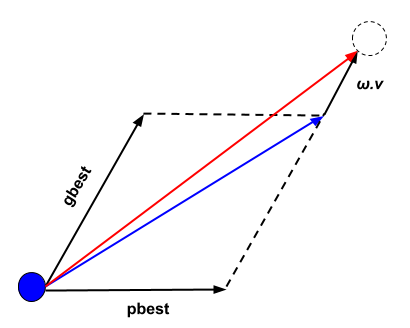
\includegraphics[scale=.5]{img/nova_part}
\caption{Atualização da posição da partícula no PSO}
\end{figure}

A constante $\omega$ ({\em ponderação de inércia}) tem por objetivo servir como um mecanismo para controlar as capacidades de diversificação e intensificação das novas partículas geradas pelo algoritmo. Basicamente, a ponderação de inércia atribui o quanto da direção de vôo anterior irá influenciar na nova velocidade da partícula numa próxima iteração do PSO \cite{Rini_2011}.

\subsection{Representação da Partícula}
\label{sec:repr_part}

A representação de uma partícula $i$ e de dimensão $D$ no PSO é, originalmente, codificada como um vetor númerico ($X^t =[x^t_1, x^t_2, x^t_3, ... ,x^t_D]$) que representa a posição (no espaço de busca) da partícula $X^t$ no instante (interação) $t$. Associado a esse vetor posição, tem-se o vetor velocidade $V^t =[v^t_1, v^t_2, v^t_3, ... , v^t_D]$ da partícula no instante $t$ que é frequentemente ajustado em cada iteração do algoritmo.

\subsection{PSO Combinatorial}
\label{sec:pso_discretos}

Devido a sua essência originalmente contínua, o PSO é normalmente relacionado à problemas contínuos \cite{Kennedy_1997}. Segundo \citeonline{Rosendo_2010}, ainda existem poucas aplicações de PSO destinadas à problemas discretos, dado, em grande parte, à sua natureza inicial contínua. 

Contudo, em razão do bom desempenho apresentado pelo algoritmo PSO na resolução de problemas de otimização de natureza contínua, intensificaram as pesquisas relacionadas à aplicação deste algoritmo na resolução de problemas de natureza combinatorial \cite{Wang2_2011}. 

A primeira abordagem embasada no PSO para domínios discretos, chamada de DPSO (\textit{Discrete Particle Swarm Optimization}), foi proposta por \citeonline{Kennedy_1997} e apresenta estrutura bastante similar à versão original do PSO. Diferentemente do PSO original, o DPSO nunca alcançou o mesmo sucesso do PSO \cite{Hoffmann_2011}. 

Nesta abordagem a velocidade da partícula continua sendo representada de forma contínua. Por outro lado, a codificação da ``posição'' adota uma representação binária, cujo valor da $i$-ésima dimensão da partícula na iteração $t+1$, é determinada através da Eq. \ref{eq:dpso_pos_bin}. A Eq. \ref{eq:dpso_sig} representa uma função sigmoidal.

\begin{equation}
\label{eq:dpso_pos_bin}
X^{t+1}_{i} = \left\{\begin{array}{l}
1\ ,\ se\ rand > S(V^{t+1}_{i}); \\
0\ ,\ senão.
\end{array}\right.
\end{equation}

\begin{equation}
\label{eq:dpso_sig}
S(x) = \frac{1}{1 + e^{-x}}
\end{equation}

Segundo \citeonline{Wang3_2011}, as aplicações envolvendo algoritmo PSO para problemas de natureza combinatorial dividem-se nas seguintes categorias: 

\begin{itemize}
\item \textbf{Baseado em representação binária}: inspirada pelo trabalho de \citeonline{Kennedy_1997}. Utiliza a representação binária na codificação da posição da partícula;
\item \textbf{Baseada em permutação}: geralmente as partículas são representadas por uma sequência ordenada de símbolos. Neste modelo, a operação de troca de posições é implementada pelo PSO para geração de novas soluções candidatas.
\end{itemize}

Alguns trabalhos que envolvem a aplicação do algoritmo PSO em problemas de classificação de dados estão relacionados na seção \ref{sec:trabalhos_relacionados}. Normalmente, os autores adotaram a representação binária na implementação do seu algoritmo, diferentemente da representação desenvolvida neste trabalho que segue a representação baseada em permutação, de acordo com a formulação proposta por \citeonline{Pan_2008}.

\subsubsection{PSO Baseado em Permutação}
\label{sec:atual_part}

No contexto de PSOs baseados em permutação, \citeonline{Pan_2008} propõem uma nova abordagem de PSO. Nesta abordagem, o processo de atualização da posição da partícula, descrito pela fórmula da Eq. \ref{eq:dpso_pos_permut}, envolve os seguintes componentes: 

\begin{equation}
\label{eq:dpso_pos_permut}
X^{t}_{i} = c_2 \otimes F_3 (\overbrace{c_1 \otimes F_2 (\underbrace{w \otimes F_1 (X^{t-1}_{i})}_{\lambda},\ pbest^{t-1}_{i})}^{\delta},\ 
gbest^{t-1})
\end{equation}

\begin{itemize}
\item O \textbf{primeiro componente} $\lambda = w \otimes F_1(X^{t-1}_{i})$ representa a velocidade da partícula. $F_1$ representa um mecanismo de busca local que ocorre segundo uma probabilidade $r_1$. Deste modo, seja $r_1$ um número aleatório gerado no intervalo de $[0,1]$, se $r_1$ for menor que $w$, então $\lambda  = F_1(X^{t-1}_{i})$. Caso contrário, $\lambda = X^{t-1}_{i}$; 

\item O \textbf{segundo componente} $\delta = c_1 \otimes  F_2(\lambda,\ pbest^{t-1}_{i})$ compreende o ``termo cognitivo'' do PSO original. $F_2$ representa um operador de recombinação ({\em crossover}) com probabilidade de ocorrer a partir de um valor aleatório $r_2 \in [0,1]$. Assim, caso $r_2$ seja menor que o parâmetro $c_1$, então $\delta = c_1 \otimes  F_2(\lambda,\ pbest^{t-1}_{i})$. Caso contrário, $\delta = \lambda$. É importante mencionar que $\lambda$ e $pbest^{t-1}_{i}$ correspondem as soluções pais da operação de recombinação; 

\item O \textbf{terceiro componente} $X^{t}_{i} = c_2 \otimes F_3 (\delta,\ gbest ^{t-1})$ compreende o ``termo social'' do PSO. $F_3$ representa um operador de recombinação em que $\delta ^{t}_{i}$ e $gbest^{t-1}$ representam as soluções pais. Assim, se um número aleatório $r_3$ for menor que o parâmetro $c_2$, então $X^{t}_{i} = c_2 \otimes F_3 (\delta,\ gbest ^{t-1})$. Caso contrário, $X^{t}_{i} = \delta$.
\end{itemize}

Onde $\lambda$ e $\delta$ são partículas temporárias utilizadas para simplificar o processo de atualização de cada partícula do enxame e $w$, $c_1$ e $c_2$ são parâmetros definidos no intervalo $[0,1]$.

%A Eq. \ref{eq:dpso_pos_permut} é implementada pelo Algoritmo \ref{alg:mdpso_atualiza_part}, apresentado na seção \ref{sec:mdpso_atual_pos_part}.

O mecanismo de \citeonline{Pan_2008}, implementado pelo PSO proposto neste trabalho e detalhado na seção \ref{sec:mdpso_atual_pos_part}, utiliza uma abordagem semelhante à formulação descrita pela Eq. \ref{eq:dpso_pos_permut}. Adaptações foram necessárias para aplicação do PSO no problema estudado neste trabalho.


\subsection{Geração da População Inicial}
\label{sec:ger_inicial}

Geralmente, as populações iniciais dos algoritmos evolucionários são construídas a partir da geração aleatória dos indivíduos (soluções candidatas) de maneira a constituir uma amostra representativa do espaço de busca. Entretanto, conforme afirmam \citeonline{Haubelt_2005}, despender um esforço inicial na implementação de heurísticas para construção das soluções iniciais de uma população pode auxiliar os algoritmos a convergirem mais rapidamente. 

Diante deste fato, o PSO proposto neste trabalho também implementa uma estratégia para construção do enxame inicial com o objetivo de auxiliar na convergência do algoritmo. A seção \ref{sec:mdpso_ger_inicial} descreve a rotina de geração do enxame inicial implementada pelo PSO proposto neste trabalho.

\subsection{Técnicas de Nicho}
\label{sec:tec_nicho}

A aplicação de técnicas de nicho pelos algoritmos populacionais consiste na divisão da população de soluções candidatas em diversas subpopulações (nichos). No contexto de problemas de classificação de dados, esta divisão da população em nichos ocorre de maneira que cada subpopulação (nicho) identifique as melhores regras de classificação de determinada classe da base de dados. Especificamente para este tipo de problema, o número de nichos é sempre igual ao número de classes.

Segundo \citeonline{Pereira_2014}, técnicas de nicho são uma funcionalidade importante, pois permitem ao algoritmo obter, simultaneamente, boas regras para as diversas classes do problema, em uma única execução. Além disso, o custo computacional total é reduzido em comparação com execuções múltiplas de uma versão do algoritmo que implemente uma população de soluções candidatas que descrevem uma única classe.

\section{Otimização Multiobjetivo}
\label{sec:multi_obj}

De acordo \citeonline{Cunha_2014}, muitos problemas encontrados na natureza são modelados como sendo de múltiplos objetivos e neste sentido, diversos esforços têm sido empregados na construção de versões multiobjetivo de Algoritmos Evolucionários para resoluções de tais problemas.

Normalmente, em problemas multiobjetivo não existe somente uma solução para o problema, mas sim um conjunto de soluções. Elas relacionam os ``{\em trade-off}'' entre os vários objetivos, e portanto, necessitam da utilização de uma noção de otimalidade para identificação destes conjuntos de soluções. 

Por isso, para problemas multiobjetivo é comum a utilização do conceito de otimalidade proposto por Francis Ysidro Edgeworth (em 1881) para comparação das soluções do problema. Este conceito difundido, posteriormente, por Vilfredo Pareto (em 1896), é denominado de {\em Edgeworth-Pareto ótimo} ou, simplesmente, {\em Pareto ótimo} \cite{Coello_2006}. Neste trabalho, é utilizado pelo PSO proposto na identifição das soluções consideradas ótimas para o problema de classificação de dados.

Frequentemente, os problemas multiobjetivo se caracterizam pela maximização (ou minimização) de um vetor de objetivos, sendo descrito por um modelo matemático conforme apresentado na formulação \ref{eq:multi_obj}:

\begin{equation}
\label{eq:multi_obj}
\textbf{Maximizar/Minimizar}\ \mathcal{F}(x) = [f_1(x),f_2(x),...,f_m(x)] \
\end{equation} 

\begin{equation}
\label{eq:sujeito_a}
\textbf{Sujeito a}\ x \in \Omega
\end{equation}

Tal que $\Omega$ é o espaço de decisões. Sejam  $u = (u_1,u_2,...,u_m)$ e $v = (v_1,v_2,...,v_m)$ tal que $u,v \in \mathbb{R}^m$. Diz-se que $u$ domina $v$, ou $u \prec v$, se $\forall u_i \leq v_i$ (problema de minimização), para todo $i=1,2,...,m$, e $\exists\ u_i < v_i$, respeitando, se existir, as restrições do problema. Quando $u$ não domina e nem é dominado por $v$, diz-se que ambos $u$ e $v$ não possuem relação de dominância entre si ou são incomparáveis.

Baseado no conceito de relação de dominância apresentado é possível aplicar a condição de otimalidade em problemas de otimização multiobjetivo. Com isso, a região de soluções viáveis $S$, tal que uma solução $x \in S$, é identificada como {\em Pareto-ótima} ou não-dominada, se e somente se, não existir outra solução $x' \in S$ tal que:

\begin{equation}
\label{eq:dominancia}
\mathcal{F}(x) \prec \mathcal{F}(x')
\end{equation}

Logo, um {\em Conjunto Pareto-Ótimo} $\mathcal{P}$ é definido por:

\begin{equation}
\label{eq:conj_pareto}
\mathcal{P} = \{x \in S, \nexists\ x' \in S\ |\ \mathcal{F}(x) \prec \mathcal{F}(x')\}
\end{equation}

Quando mapeadas no espaço dos objetivos, as {\em soluções Pareto-ótimas} são chamadas de {\em Fronteira Pareto}, $\mathcal{PF}$. Ou seja:

\begin{equation}
\label{eq:front_pareto}
\mathcal{PF} = \{ u = \mathcal{F}(x)\ |\ x \in \mathcal{P} \}
\end{equation}

A tarefa de encontrar a fronteira Pareto exata de um problema de otimização multiobjetivo pode ser difícil. Dessa maneira, são aceitáveis aproximações de uma fronteira Pareto encontradas dentro de um intervalo limitado de processamento computacional \cite{Coello_2006}. Tais soluções devem estar o mais próximo da fronteira Pareto real com a maior diversidade possível de amostras. 

A otimização multiobjetivo é uma importante área de pesquisa para cientistas e engenheiros. Técnicas tradicionais de otimização, tais como métodos baseados em gradientes, são difíceis, senão impossíveis, de serem utilizados em verdadeiros problemas de otimização multiobjetivo. Devido a isso, abordagens evolucionárias têm sido desenvolvidas para serem aplicadas na resolução de problemas de otimização multiobjetivo \cite{Hu_2003}. 

A classificação de dados por meio de extração de regras, tema deste trabalho, é formulada como um problema de otimização. Conforme afirma \citeonline{Liu_2004}, problemas de otimização multiobjetivo podem ser reduzidos à problemas de classificação de dados, cujo objetivo principal é encontrar regras de classificação com alta precisão, generalização e compreensão. 


\subsection{PSO Multiobjetivo}
\label{sec:pso_mult}

A relativa simplicidade do PSO, em conjunto com suas técnicas de compartilhamento de informação, tornaram-o um candidato natural para desenvolvimento de uma variante do PSO para aplicação em problemas de natureza multiobjetivo \cite{Mishra_2016}. Entretanto, apesar do PSO se mostrar particularmente adequado à abordagem multiobjetivo, devido ao seu poder de convergência para problemas mono-objetivo \cite{Coello_2004}, parece que ainda não há um consenso acerca da melhor forma de representação dos componentes {\em gbest} e {\em pbest} no contexto multiobjetivo \cite{Reddy_2007}. 

Cabe ressaltar que, na versão mono-objetivo do PSO, os componentes {\em pbest} e {\em gbest} representam uma solução somente. Porém, no contexto da otimização multiobjetivo, a representação de {\em pbest} e {\em gbest} é uma questão a ser analisada, visto que tais componentes passam a se comportar como um repositório, contendo inúmeras soluções não-dominadas.

\section{Busca Local Pareto}
\label{sec:busca_local_pareto}

Os mecanismos de busca local são conhecidos pela sua eficiência em várias situações práticas, especialmente em problemas combinatórios complexos \cite{Basseur_2007}. A introdução destes mecanismos em algoritmos multiobjetivo é relativamente comum uma vez que eles possibilitam a esses algoritmos convergirem mais rapidamente e com mais precisão em direção à fronteira Pareto \cite{Joao_2013}.

Normalmente, estes mecanismos tentam aprimorar, iterativamente, uma solução $s$ através de sucessivas substituições da solução corrente por uma solução melhor (solução mutante) encontrada na vizinhança da solução $s$. A vizinhança de uma solução $s$, representada por $\mathcal{N}(s)$, compreende ao conjunto de soluções (chamados vizinhos) que podem ser alcançados a partir de $s$ através de modificações ou perturbações (operações de {\em move}) na solução corrente $s$ \cite{Zachariadis_2010}.

Os algoritmos de {\em busca local Pareto} (PLS, {\em Pareto Local Search}) são técnicas de busca local nas vizinhanças de uma solução para resolução de problemas de otimização combinatorial multiobjetivo. As PLSs aplicam uma estratégia de exploração iterativa em um conjunto de soluções, objetivando obter consequentemente novas soluções não-dominadas, a partir de pesquisas nas vizinhanças de cada solução do conjunto \cite{Drugan_2012}. 

Os métodos de busca local Pareto propostos por  \citeonline{Drugan_2012} são descritos nas seções seguintes e têm em comum os seguintes parâmetros: uma solução inicial $s$, um conjunto de soluções não-dominadas $A$ e uma função multiobjetivo $\mathcal{F}(x)=[f_1(x), f_2(x), \dots, f_m(x)]$. Ao final da execução de cada método, é retornado o conjunto de soluções não-dominadas $A'$.

\subsection{Best Pareto Improvement - BPI} 

Descrito no Algoritmo \ref{alg:BPI}, o {\em Best Pareto Improvement} (BPI) varre toda a vizinhança da solução $s$. O conjunto de soluções $A’$ contém as soluções encontradas na vizinhança $\mathcal{N}(s)$ que dominam ou são incomparáveis com as soluções do conjunto $\{s\} \cup A$. 

O parâmetro {\em visited} identifica se a vizinhança de determinada solução já foi examinada anteriormente pelo método ({\em visited} = TRUE) ou não ({\em visited} = FALSE). O atributo {\em visited} de cada solução é inicializado com valor FALSE.

\begin{algorithm}[H]
\caption{Best Pareto Improvement}
\label{alg:BPI}
\begin{algorithmic}[1]
\INPUT{$s$ - Solução inicial; $A$ - Conjunto Pareto de entrada.}
\State $A' \leftarrow \{s\} \cup A$;
\For{$s' \in \mathcal{N}(s)$} 
  \If{$\forall s'' \in A',f(s') \prec f(s'') \vee f(s') \parallel f(s'')$} // $\parallel$ - \small{não há relação de dominância}
    \State $s'.visited \leftarrow$ FALSE;
    \State $A' \leftarrow merge(A', \{s'\})$;
  \EndIf
\EndFor
\State $A' \leftarrow A' \setminus (\{s\} \cup A)$;
\State \Return $A'$;
\end{algorithmic}
\end{algorithm}

A função {\em merge} (linha 4) agrupa os dois conjuntos Pareto em um novo conjunto Pareto, removendo as soluções dominadas do conjunto resultante. No método BPI, as buscas na vizinhança de uma solução $s$ envolvem todas as soluções do conjunto $A'$ que não tenham sido visitadas ($visited$ = FALSE).

\subsection{First Pareto Improvement - FPI} 

Descrito no Algoritmo \ref{alg:FPI}, o processo de busca na vizinhança pelo método {\em First Pareto Improvement} (FPI) é finalizado quando a primeira solução localizada em $\mathcal{N}(s)$ que domina a solução corrente $s$ é encontrada.

\begin{algorithm}[H]
\caption{First Pareto Improvement}
\label{alg:FPI}
\begin{algorithmic}[1]
\INPUT{$s$ - Solução inicial; $A$ - Conjunto Pareto de entrada.}
\State $A' \leftarrow \{s\} \cup A$;
\For{$s' \in \mathcal{N}(s)$} 
  \If{$\forall s'' \in A',f(s') \prec f(s'') \vee f(s') \parallel f(s'')$}
	\State $s'.visited\leftarrow$ FALSE;
    \State $A' \leftarrow merge(A', \{s'\})$;
    \If{$f(s') \prec f(s)$}
      \State $A' \leftarrow A' \setminus (\{s\} \cup A)$;
      \State \Return $A'$;
    \EndIf
  \EndIf
\EndFor
\State $A' \leftarrow A' \setminus (\{s\} \cup A)$;
\State \Return $A'$;
\end{algorithmic}
\end{algorithm}

\subsection{Neutral Pareto Improvement - NPI} 

O método {\em Neutral Pareto Improvement} (NPI), apresentado pelo Algoritmo \ref{alg:NPI}, interrompe a busca na vizinhança da solução $s$ quando um vizinho que não é dominado nem pela solução corrente $s$ e tampouco por nenhuma solução do conjunto $A$ é identificado.

\begin{algorithm}[H]
\caption{Neutral Pareto Improvement}
\label{alg:NPI}
\begin{algorithmic}[1]
\INPUT{$s$ - Solução inicial; $A$ - Conjunto Pareto de entrada.}
\State $A' \leftarrow \{s\} \cup A$;
\For{$s' \in \mathcal{N}(s)$} 
  \If{$\forall s'' \in A',f(s') \prec f(s'') \vee f(s') \parallel f(s'')$} 
    \State $s'.visited \leftarrow$ FALSE;
    \State $A' \leftarrow merge(A', \{s'\})$;
    \State $A' \leftarrow A' \setminus (\{s\} \cup A)$;
    \State \Return $A'$;
  \EndIf
\EndFor
\State \Return $\emptyset$;
\end{algorithmic}
\end{algorithm}

\section{Mineração de Dados}
\label{sec:md}

Os avanços da tecnologia têm produzido uma abundância de dados. Logo, empregar métodos e técnicas capazes de analisar e extrair conhecimento de bases de dados tem se tornado um fator importante à tomada de decisões. De acordo com \citeonline{Fayyad_1996}, por meio de KDD ({\em Knowledge Discovery in Database})\footnote{Tradução: Descoberta de conhecimento em banco de dados}, é possível extrair informações implícitas, não triviais, previamente desconhecidas e potencialmente úteis em um banco de dados, que muitas vezes são inutilizadas ou pouco aproveitados dentro do ambiente de trabalho. 

A {\em mineração de dados} ({\em data mining}) é uma fase dentro do processo de KDD e consiste basicamente na aplicação de algoritmos que, sob aceitável eficiência computacional, possam contribuir no reconhecimento de padrões, ou modelos, acerca dos dados estudados \cite{Fayyad_1996_2}. 

Nos dias de hoje, a mineração de dados tem despertado a atenção de diversos estudiosos, sendo citada pelos mesmos como um elemento fundamental em pesquisas relacionadas a área estratégica industrial, já que permite extrair informações que alavanquem seus negócios bem como a descoberta de novas oportunidades de inovação \cite{Chen_1996}.

O termo mineração de dados foi cunhado em alusão ao processo de mineração, isto é, o processo de extração de minerais preciosos, que pode ser compreendido da seguinte maneira: explora-se uma base de dados (mina) usando algoritmos (ferramentas) para a obtenção de conhecimento (minerais preciosos) \cite{Castro_2016}. 

Diversas tentativas têm sido utilizadas na aplicação de algoritmos evolucionários para a realização das tarefas de mineração de dados. Neste contexto, o PSO se apresenta como uma ferramenta promissora na aplicação em problemas de mineração de dados devido a sua facilidade de implementação e poucos parâmetros a serem ajustados \cite{Wang_2007}, sendo considerado um método robusto à resolução de problemas não-lineares, não-integráveis, multimodais e de alta dimensionalidade \cite{Krohling_2004}. 


\subsection{Classificação de Dados}
\label{sec:classif_dados}

Classificar um objeto significa atribuir um rótulo, chamado {\em classe}, de acordo com a categoria à qual ele pertence. Para que isso seja possível, um algoritmo ou método é utilizado na construção de um modelo de classificação - também chamado de {\em classificador}. Existe uma variedade de algoritmos destinados à tarefa de classificação de dados na literatura, como por exemplo as {\em Árvores de Decisão}, as {\em Rede Neurais Artificiais}, {\em Máquina de Vetores Suporte}, {\em Algoritmos Evolucionários}, etc, cujas aplicações incluem a identificação de {\em spams}, atribuição de crédito e detecção de fraudes, além de outras \cite{Castro_2016}.

A {\em extração de regras} (do inglês {\em rule mining} ou {\em rule discovery}) é um método dentro da classificação de dados que busca encontrar um conjunto de regras {\em SE-ENTÃO} para classificar, de forma mais ``natural'',  uma base de dados. Conforme explica \citeonline{Pereira_2012}, a extração de regras é um tópico recorrente na mineração de dados, segundo \citeonline{Hassani_2013}, caracterizado por ser um problema {\em NP-Completo}.

Cabe observar que a obtenção de regras com alto grau de precisão na etapa de treinamento não é garantia de que o mesmo sucesso seja obtido na fase de testes. Isso ocorre pelo fato de que regras muito adaptadas a um determinado conjunto de dados tendem a ser ineficientes na classificação de novos dados ({\em overfitting})\footnote{Tradução: Sobregeneralização}, sendo incapazes de promover a generalização \cite{Pereira_2010}. 

Deste modo, buscar um conjunto de regras que seja o mais simples (com menor número de termos) também é um objetivo normalmente explorado por alguns algoritmos que abordam o problema de classificação de dados (\citeonline{Pereira_2014}, \citeonline{Liu_2004}, \citeonline{Sousa_2004}, etc).

A Figura \ref{fig:modeloPSO} ilustra as diversas etapas presentes no processo de classificação de dados através de conjunto de regras {\em SE-ENTÃO}: 

\begin{enumerate}[label={(\roman*)}]
\item Fase de coleta de dados;
\item Extração das regras de classificação que ocorre durante a fase de treinamento;
\item Construção do modelo de classificação;
\item Classificação de novas amostras que ocorre na fase de testes.
\end{enumerate}

\begin{figure}[ht]
\centering
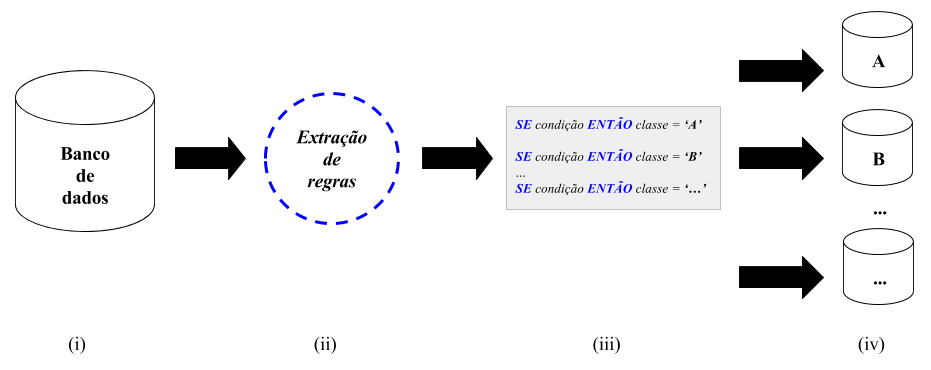
\includegraphics[scale=.4]{img/modelo}
\caption{Etapas que compõem a classificação de dados através de um conjunto de regras {\em SE-ENTÃO}.}
\label{fig:modeloPSO}
\end{figure}

Abordagens não-baseadas em extração de regras {\em SE-ENTÃO} apesar de representarem o conhecimento descoberto, funcionam como modelos de ``caixa preta'' e tendem a apresentar baixa compreensão, mesmo possuindo elevados níveis de precisão. São exemplos de métodos de classificação não-baseados em regras: {\em Máquinas de Suporte Vetorial} e {\em Redes Neurais Artificiais}, que mesmo apesar de apresentarem níveis de previsão considerados ótimos, são de  difícil compreensão \cite{Hassani_2013}. Por outro lado, abordagens baseadas em regras {\em SE-ENTÃO} são mais intuitivas, já que tendem a beneficiar a representação simbólica do conhecimento, facilitando a sua compreensão por parte dos usuários \cite{Wang_2007}.

Uma regra {\em SE-ENTÃO} é composta basicamente por dois componentes: os {\em antecedentes} (ou restrições) e os {\em consequentes} (a classe predita), conforme ilustrado no esquema da Figura \ref{fig:se-entao}.

\begin{figure}[ht]
\centering
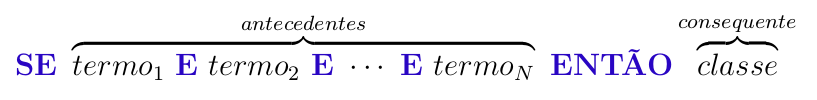
\includegraphics[scale=.5]{img/se-entao}
\caption{Estrutura das regras {\em SE-ENTÃO}.}
\label{fig:se-entao}
\end{figure}

Os {\em antecedentes} são um conjunto de termos, em que cada termo é descrito por uma tríade com a seguinte estrutura: \textit{<atributo, operador, valor numérico ou outro atributo>}, conectados por conectores lógicos \textbf{E} ({\em AND}), formando consequentemente uma série de restrições (condições) que devem ser atendidas. O {\em consequente} é posicionado após a cláusula \textbf{ENTÃO} da regra e define a classe que é predita pela regra. Em resumo, se os dados da base satisfazem os antecedentes, então estes são identificados com a classe associada à regra.

Para \citeonline{Freitas_2003} há duas abordagens para representação das regras pelos algoritmos evolucionários propostos para problemas de classificação de dados:
 
\begin{itemize}
\item \textbf{Abordagem Pittsburgh}: O indivíduo representa um conjunto de regras. Esta representação possui maior dificuldade de formulação e implementação pelos algoritmos;
\item \textbf{Abordagem Michigan}: Cada indivíduo representa uma única regra. Esta representação é mais fácil de implementar e tende a reduzir o tempo de cálculo da aptidão ({\em fitness}) do indivíduo.
\end{itemize}

Normalmente, os algoritmos para problemas de classificação de dados raramente utilizam a abordagem Pittsburgh. De acordo \citeonline{Cervantes_2005}, a abordagem Michigan apresenta certas vantagens em relação à abordagem Pittsburgh, como: (i) capacidade de fornecer boas soluções com um número menor de avaliações da função-objetivo e (ii) maior flexibilidade na representação das regras de classificação.

A classificação de dados por meio de extração de regras estudada neste trabalho é modelada como um problema de otimização biobjetivo em que se busca maximizar a efetividade das regras extraídas ao mesmo tempo em que se tenta minimizar a complexidade das regras (tamanho), uma vez que regras menores são mais simples de serem entendidas e tendem a evitar o {\em overfitting} \cite{Pereira_2012}.

\subsection{Avaliação da Classificação de Dados}
\label{sec:aval_fit}

Entende-se como ``qualidade'' de uma regra a capacidade em classificar corretamente o maior número de padrões (ou registros) de um banco de dados. Existem diversas formas de se medir a qualidade de uma regra de classificação, sendo que as mais comuns se baseiam em cálculos realizados a partir dos coeficientes da matriz de confusão (Ver Tabela \ref{tab:matriz_confusao}) \cite{Pereira_2012}.

% http://tex.stackexchange.com/questions/9253/slashbox-alternative
\begin{table}[!ht]
	\centering
 	\begin{tabularx}{\linewidth}{
    |>{\hsize=.33 \hsize}X|
    >{\hsize=.33 \hsize}X|
    >{\hsize=.33 \hsize}X|
  	}
 	\hline \diagbox[width=12.8em]{ \textbf{Real} }{ \textbf{Classif.} } & \textbf{Positivo} & \textbf{Negativo} \\
 	\hline \textbf{Positivo} & {\em Verdadeiro Positivo} (VP) & {\em Falso Negativo} (FN) \\
    \hline \textbf{Negativo} & {\em Falso Positivo} (FP)      & {\em Verdadeiro Negativo} (VN) \\
 	\hline 
	\end{tabularx}
	\caption{Matriz de confusão}
	\label{tab:matriz_confusao}
\end{table}

Os coeficientes presentes na matriz permitem o cálculo de importantes métricas para averiguar o desempenho dos classificadores. São exemplos: a {\em acurácia} (Eq. \ref{eq:acuracia}), {\em sensibilidade} (Eq. \ref{eq:sensibilidade}) e {\em especificidade} (Eq. \ref{eq:especificidade}), dentre outras:

\begin{equation}
\label{eq:acuracia}
Acurácia = \frac{VP + VN}{VP + FN + FP + VN}
\end{equation}

\begin{equation}
\label{eq:sensibilidade}
Sensibilidade = \frac{VP}{VP + FN}
\end{equation}

\begin{equation}
\label{eq:especificidade}
Especificidade = \frac{VN}{VN + FP}
\end{equation}

Onde:

\begin{itemize}
\item \textbf{Verdadeiros positivos} (VP): total de registros (ou tuplas) recuperados do banco de dados utilizando a regra codificada nas quais os respectivos registros coincidem com a classe predita; 

\item \textbf{Falsos positivos} (FP): total de registros recuperados pela regra e que não pertecem à classe predita;

\item \textbf{Verdadeiros negativos} (VN): total de registros que não são cobertas pela regra e que não pertença à classe; 

\item \textbf{Falsos negativos} (FN): total de registros que não foram obtidas pela regra, mas que pertencem à classe predita.
\end{itemize}

\section{Trabalhos Relacionados}
\label{sec:trabalhos_relacionados}

A tarefa de classificação de dados pode ser realizada por meio de diversas abordagens. A seguir são apresentados trabalhos relevantes encontrados no contexto de classificação de dados por meio de PSO que serviram de referência para desenvolvimento desse trabalho.

\citeonline{Sousa_2004} apresentam um estudo acerca de uma variante do PSO destinada à classificação de dados por meio da extração de regras {\em SE-ENTÃO} numa abordagem mono-objetivo, sendo a aptidão das partículas avaliadas a partir do cálculo do produto da sensibilidade pela especificidade. É interessante notar que as partículas, posteriormente à avaliação de aptidão, passam por uma fase de encolhimento ({\em prunning}), com o objetivo eliminar os atributos que não contribuem para eficácia da regra. O trabalho investiga as seguintes variantes do PSO: {\em Discrete PSO} (DPSO), {\em Constricted PSO} (CPSO) e {\em Linear Decreasing Weight PSO} (LDWPSO).

\citeonline{Liu_2004} apresentam um classificador baseado no PSO para classificação de dados chamado de {\em Rule Discovery with Particle Swarm Optimization} (REPSO). Neste classificador, cada partícula representa uma única regra e, segundo os autores, tem a vantagem de poder ser aplicada tanto em dados categóricas como em dados contínuos. Durante os testes, foram utilizadas duas bases de dados do {\em UCI repository of Machine Learning}: a base de dados {\em Zoo}, no qual todos os atributos são categóricos e o conjunto de dados {\em Wine}, no qual todos os atributos, exceto o atributo de classificação, são contínuos. As regras descobertas pelo algoritmo foram avaliadas pelo somatório da acurácia obtida e pelo número de termos utilizado pela regra, sendo atribuídos ``pesos'' a cada um, na avaliação da aptidão ({\em fitness}) da solução.

\citeonline{Cervantes_2005} avaliam o desempenho de um PSO binário para classificação de dados utilizando as abordagens Pittsburgh e Michigan na codificação das partículas. O PSO proposto no trabalho apresenta as seguintes adaptações: (i) a adição de uma força competitiva que repele uma partícula de seu melhor vizinho e (ii) a utilização de vizinhanças dinâmicas baseadas num critério de proximidade. Os resultados obtidos mostraram que a abordagem Michigan foi superior à abordagem Pittsburgh na maioria das situações analisadas pelo artigo.

\citeonline{Zahari_2007} propõem um classificador PSO inteligente chamado de {\em Intelligent Particle Swarm Classifier} (IPS-{\em classifier}). Este classificador tenta encontrar hiperplanos de decisão para determinação das diferentes classes dentro do espaço de busca. Um controlador {\em fuzzy} foi também projetado para melhorar o desempenho e eficiência do classificador proposto, adaptando os parâmetros de ponderação de inércia e os fatores cognitivo e social do PSO. 

\citeonline{Wang2_2011} propõem um algoritmo mono-objetivo para classificação de dados e mineração de regras utilizando o DPSO. As regras são codificadas através de uma cadeia de {\em bits} de comprimento fixo, em que o número de termos utilizados pela regra é ajustado dinamicamente por meio de um {\em bit} adicional para cada termo com objetivo de determinar a sua existência, ou não, em determinada regra. Nesta proposta, cada partícula é representada por um grupo de regras (abordagem Pittsburgh) e os resultados obtidos mostraram que o PSO proposto alcançou maior acurácia e uma lista de regras menor do que outros algoritmos analisados pelo artigo.

\citeonline{Chen2_2012} apresentam uma implementação DPSO, chamada de {\em Discrete Particle Swarm Optimization With Local Search} (DPSO-LS), que utiliza a abordagem Pittsburgh para codificação da partícula. Cada partícula do enxame é representada por uma matriz em que cada linha descreve uma regra de classificação {\em SE-ENTÃO} durante a tarefa de classificação de dados. Além disso, avaliou-se neste trabalho a importância da utilização de técnicas de busca local para refinamento dos resultados encontrados.

\citeonline{Hassani_2013} apresentam um DPSO para mineração de regras de classificação que utiliza uma separação dos dados de treinamento em blocos em que cada um é atribuído a uma {\em thread}. Ao final, as regras obtidas em cada {\em thread} são integradas em uma base de regras para construção de um modelo de classificação.

\citeonline{Mishra_2016} apresenta um classificador para mineração de regras de associação com abordagem multiobjetivo para maximização do {\em suporte} ({\em cobertura}) e {\em confiança} da regra de associação ao mesmo tempo em que tenta minimizar a complexidade da mesma.

A maioria dos trabalhos relacionados acima propõem estruturas de dados baseadas em uma representação binária das partículas para extração de regras de classificação ou associação, similares ao DPSO proposto por \citeonline{Kennedy_1997}. 

Em problemas de classificação de dados que levam em consideração a complexidade das regras são utilizados mecanismos para ignorar certos termos da regras {\em SE-ENTÃO} codificadas nas partículas. Geralmente, estas codificações envolvem a utilização de um vetor com todos os atributos da base de dados e um {\em bit} que habilita ou não a utilização de determinado atributo na regra. Neste contexto, o seguinte trabalho se torna relevante ao utilizar uma nova abordagem baseada no trabalho de \citeonline{Pan_2008} (Ver seção \ref{sec:atual_part}) para codificação e atualização da posição da partícula.

\citeonline{Pan_2008} propõem um processo de atualização da posição da partícula alternativo. Neste estudo, o PSO proposto é aplicado em ambientes combinatoriais na resolução de problemas de alocação de recursos e escalomanento ({\em flow-shop}). De acordo os autores, tal abordagem pode ser facilmente aplicada em problemas de otimização combinatorial com resultados que demonstram ser competitiva, podendo inclusive obter resultados superiores a outros métodos encontradas na literatura especializada.

Finalmente, cabe também mencionar o trabalho de \citeonline{Pereira_2012} que serviu de embasamento na utilização da metodologia aplicada durante à análises dos resultados. No seu trabalho é proposto uma variante multiobjetiva baseada em Programação Genética (PG) para extração de regras de classificação, sendo realizadas comparações de desempenho com três algoritmos implementados pelo WEKA.

\section{Conclusão}

Neste capítulo, foram apresentados os principais conceitos e definições relacionados ao PSO. Fez-se uma descrição de suas características principais, ressaltando suas funcionalidades e aplicações. Em seguida, foram relacionadas variantes do PSO destinadas ao ambiente combinatorial e as estratégias de geração do enxame inicial e técnicas de nicho.

Conceitos relacionados a otimização multiobjetivo, busca local Pareto e mineração de dados (classificação de dados), bem como a apresentação de estudos relevantes que serviram de referência para este trabalho também foram apresentados. Nota-se que ainda existem poucos que utilizam o PSO para a classificação de dados por meio da extração de regras. Não foi encontrado nenhum trabalho de classificação de dados baseado em PSO utilizando a formulação proposta por \citeonline{Pan_2008}, o que torna o presente trabalho inovador neste sentido.

% ---------
% Proposta 
% ---------

\chapter{mDPSO - Algoritmo Biobjetivo baseado em PSO para Classificação de Dados}
\label{ch:mdpso}

Neste capítulo será detalhado o algoritmo biobjetivo, baseado na metaheurística PSO e denominado {\em multiobjective Discrete Particle Swarm Optimization} (mDPSO) proposto neste trabalho para classificação de dados por meio de extração de regras. 

Ao contrário de outras variantes do algoritmo PSO destinadas à classificação e mineração de dados, o mDPSO utiliza uma abordagem diferente das que são comumente encontradas na literatura. Ele também implementa um conjunto de funcionalidades para explorar o espaço de busca e acelerar sua convergência.

\section{Formulação do Problema}
\label{sec:form_problema}

Neste trabalho, o problema de classificação de dados foi modelado como um problema  biobjetivo, descrito pela Eq. \ref{eq:fitness}, no qual os objetivos são: (i) maximizar a efetividade das regras extraídas; e (ii) minimizar a complexidade (número de termos) das regras. 

\begin{equation}
\label{eq:fitness}
\textbf{Maximizar}\ \mathcal{F}(x) = [f_1(I,X), f_2(I,X)]
\end{equation}

\begin{itemize}
   \item $x$ é uma sentença da cláusula WHERE da linguagem SQL;
   \item Os parâmetros $I$ e $X$ representam respectivamente a regra codificada pela partícula e a classe $X$ (nicho) a que a partícula pertence;
   \item $f_1(I,X)$, descrita por Eq. \ref{eq:fitness1}, corresponde à função que determina a efetividade (qualidade) da regra. Esta efetividade é resultante do produto da sensibilidade pela especificidade; 
   \item $f_2(I,X)$, descrita na Eq. \ref{eq:fitness2}, representa a função que calcula a complexidade da regra. Neste trabalho ela é calculada como sendo o número inverso de termos da regra.
\end{itemize}

\begin{equation}
\label{eq:fitness1}
f_1(I,X) = sensibilidade \times especificidade
\end{equation}

\begin{equation}
\label{eq:fitness2}
f_2(I,X) = \frac{1}{número\ de\ termos}
\end{equation}

De acordo com \citeonline{Pereira_2012}, o produto da sensibilidade pela especificidade apresenta propriedades interessantes, pois tende a evitar o {\em overfitting}, já que busca reduzir, ou até mesmo eliminar, a tendência de privilegiar as classes predominantes presentes em bancos de dados desbalanceados. Dessa maneira, se a regra apresentar um desempenho muito baixo em relação a um dos valores da sensibilidade ou da especificidade, o valor do {\em fitness} da partícula também será baixo, independente do outro indicador. A função {\em fitness} é penalizada por regras incapazes de identificar os padrões corretos, pois uso da acurácia pode resultar em um valor elevado, mesmo que o número de {\em verdadeiro positivos} (VP) seja alto e o valor de {\em verdadeiro negativo} (VN) seja próximo de zero. 

\section{Descrição do mDPSO}
\label{sec:desc_mdpso}

O objetivo do mDPSO é extrair um conjunto de regras durante as fases de treinamento para avaliar seu desempenho em novas amostras, desconhecidas durante a tarefa de treinamento, na fase de teste.

A abordagem Michigan foi utilizada para representação das partículas do mDPSO. Dessa maneira, cada partícula codifica apenas uma regra do problema, o que significa dizer que cada partícula provê uma solução possível para determinada classe e não uma solução geral para todo o problema. 

O mDPSO, descrito no Algoritmo \ref{alg:pseudo_mdpso}, implementa um conjunto de particularidades que o distinguem das demais implementações (variantes) da metaheuristica PSO encontradas na literatura. São funcionalidades adaptadas, implementadas pelo mDPSO:

\begin{itemize}
\item \textbf{Repositórios {\em gbest} e {\em pbest}} (Ver seção \ref{sec:rep_best});
\item \textbf{Geração do Enxame Inicial} (Ver seção \ref{sec:mdpso_ger_inicial});
\item \textbf{Implementação de um Operador de Turbulência} (Ver seção \ref{sec:mdpso_oper_turb});
\item \textbf{Atualização da Posição da Partícula} (Ver seção \ref{sec:mdpso_atual_pos_part});
\item \textbf{Operação de Mutação de Partícula} (Ver seção \ref{sec:mdpso_mutacao});
\item \textbf{Rotina de Recombinação das Partículas} (Ver seção \ref{sec:mdpso_recomb_part}).
\end{itemize}

\begin{algorithm}[ht]
\caption{mDPSO}
\label{alg:pseudo_mdpso}
\begin{algorithmic}[1]
\State Geração do enxame inicial de partículas (Ver seção \ref{sec:mdpso_ger_inicial}); 
\State Avaliar as partículas do enxame (Ver Algoritmo \ref{alg:pseudo_mdpso_aval});
\While{critério de parada não atingido}
  \State Aplicar o operador de turbulência (Ver seção \ref{sec:mdpso_oper_turb}); 
  \State Atualizar a velocidade e posição de todas partículas do enxame (Ver seção \ref{sec:mdpso_atual_pos_part});
  \State Avaliar as partículas do enxame;    
  \For{cada partícula $p \in C_k.gbest$}
	\State Aplicar busca local Pareto em $p$ (Ver seção \ref{sec:mdpso_busca_local});
	\State Avaliar $p$;
   \EndFor
\EndWhile
\end{algorithmic}
\end{algorithm}

\begin{algorithm}[ht]
\caption{Avaliação de aptidão ({\em fitness}) de cada partícula no mDPSO}
\label{alg:pseudo_mdpso_aval}
\begin{algorithmic}[1]
\INPUT{$p.pbest$ - Soluções não-dominadas encontradas pela partícula; $C_k.gbest$ - Soluções não-dominadas do nicho $C_k$}.
  \For{cada partícula $p$ do enxame}
      \State Avaliar $p$;
      \State $C_k.gbest \leftarrow merge(C_k.gbest, \{p\})$;
      \State $p.pbest \leftarrow merge(p.pbest, \{p\})$;
  \EndFor
\end{algorithmic}
\end{algorithm}

A função {\em merge}, tal como descrita na seção \ref{sec:busca_local_pareto}, agrupa dois conjuntos Pareto em um novo conjunto Pareto, removendo as soluções dominadas do conjunto resultante.

Nas próximas seções será feito o detalhamento de cada funcionalidade implementada pelo mDPSO.

\section{Representação da Partícula}
\label{sec:mdpso_repr_part}

A representação adotada para cada partícula do mDPSO é ilustrada na Figura \ref{fig:representacao} e compreende dois componentes:

\begin{itemize}
\item Um vetor de tamanho variável de elementos (termos) que codificam a regra de classificação.
\item Um rótulo identificador da classe (nicho).
\end{itemize}

Na avaliação da aptidão ({\em fitness}) da partícula no PSO, esse vetor de termos é convertido em um predicado lógico da claúsula WHERE de uma sentença SQL, conforme ilustrado na Figura \ref{fig:representacao}, quando executada em um Sistema de Gerenciamento de Banco de Dados (SGBD) que retorna os registros (tuplas) do banco que atendem à cláusula WHERE da sentença SQL. 

De posse dos registros retornados é feita a avaliação do desempenho da regra codificada na partícula.

\begin{figure}[ht]
\centering
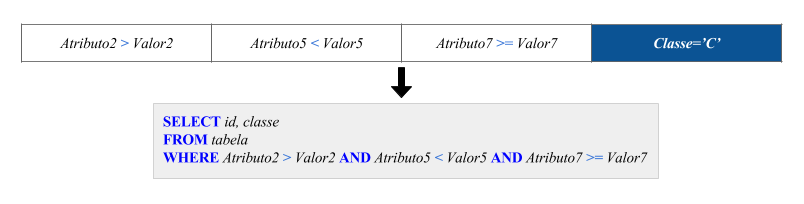
\includegraphics[scale=.5]{img/representacao}
\caption{Exemplo de codificação de uma partícula pelo mDPSO e a sentença SQL gerada para avaliação pelo SGBD.}
\label{fig:representacao}
\end{figure}


\section{Repositórios {\em gbest} e {\em pbest}}
\label{sec:rep_best}

Um ponto importante no mDPSO refere-se aos componentes {\em gbest} e {\em pbest}. Em versões multiobjetivo do PSO, ambos {\em gbest} e {\em pbest} passam a atuar como repositórios de soluções não-dominadas, ao contrário da versão mono-objetivo, em que ambas se referem somente à melhor posição obtida pela partícula ({\em pbest}) e a melhor posição obtida pelo enxame ({\em gbest}).

O mDPSO implementa o {\em gbest} através de um repositório de soluções não-dominadas para cada nicho (classe) do problema  ($C_k.gbest$). De forma semelhante, o mDPSO também representa o {\em pbest} de cada partícula como um repositório de soluções não-dominadas.  

Geralmente, o PSO implementa o conceito de partícula líder, que é utilizada na atualização das posições das partículas do enxame, isto é, uma solução que contribui no direcionamento do enxame dentro do espaço de busca. Nas versões mono-objetivo a partícula líder é o próprio {\em gbest}, sendo por isso necessária a proposição de um mecanismo de identificação da partícula líder em abordagens multiobjetivo, visto que, neste contexto, tanto o {\em gbest} quanto {\em pbest} são representadas por um repositório (conjunto) de soluções não-dominadas. 

O processo de identificação da partícula líder ({\em gbest} ou {\em pbest}), necessária à recombinação no mDPSO durante a operação de atualização da posição de cada partícula, ocorre da seguinte maneira: (i) Determina-se a distância euclidiana no plano dos objetivos da partícula corrente em relação aos repositórios {\em gbest} ou {\em pbest}; (ii) A partícula mais próxima da partícula corrente em cada repositório é selecionada para atualização da sua posição durante a recombinação. 

A escolha da partícula não-dominada  mais próxima da partícula corrente na rotina de atualização da posição é exemplificada pela Figura \ref{fig:sel_lider}. A partícula escolhida (partícula líder) é realçada na cor vermelha e a partícula corrente na cor azul.

\begin{figure}[ht]
\centering
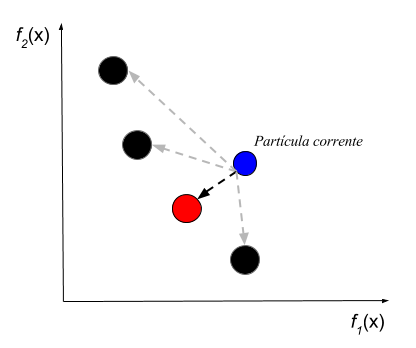
\includegraphics[scale=.5]{img/best}
\caption{Escolha da partícula líder}
\label{fig:sel_lider}
\end{figure}

Tal abordagem é implementada pelo algoritmo de recrutamento de abelhas {\em OptBees} \cite{Renato_2012}. O {\em OptBees} é um algoritmo aplicado na resolução de problemas de otimização em espaços contínuos, sendo inspirado no comportamento das abelhas durante o forrageamento e em mecanismos envolvidos no processo de alocação de tarefas da vida em sociedade do enxame. É importante também frisar que tal abordagem pode ser aplicada tanto em problemas de maximização quanto de minimização.

Cabe também ressaltar que ao final de cada iteração do mDPSO, com o objetivo de refinar ou aprimorar as soluções encontradas até aquela iteração, é proposta uma busca local Pareto (Ver seção \ref{sec:mdpso_busca_local}) no repositório {\em gbest} de cada nicho.

\section{Geração do Enxame Inicial}
\label{sec:mdpso_ger_inicial}

O mDPSO implementa uma rotina para geração inicial do seu enxame de partículas. A rotina proposta, descrita pelo Algoritmo \ref{alg:mdpso_ger_inicial}, funciona em duas etapas: (i) Primeiramente, aplica-se técnicas de nicho (Ver seção \ref{sec:tec_nicho}) para dividir o enxame segundo o número de classes do problema; (ii) Gera-se a regra de cada partícula do enxame. 

\begin{algorithm}[ht]
\caption{Geração do Enxame Inicial}
\label{alg:mdpso_ger_inicial}
\begin{algorithmic}[1]
\INPUT{$N$ - Número de partículas do enxame;}.
\State $Enxame$ $\leftarrow \emptyset$;
\For{Cada classe $C_k$ do problema}
 \State $C_k.gbest \leftarrow \emptyset$;
\EndFor
\For{cada partícula do enxame}
 \State $\eta \leftarrow \ceil[\big]{\log{(rand_{[1, N]})}} + 1$;
 \State $partícula\ \leftarrow$ Adicionar regra de $\eta$ termos;
 \State $partícula\ \leftarrow$ Rotular partícula ($C_k$);
 \State $partícula.pbest\ \leftarrow  \emptyset$;
 \State $Enxame\ \leftarrow  \{partícula\} \cup Enxame$;
\EndFor
\end{algorithmic}
\end{algorithm}

A fase de geração (linha 7 do Algoritmo \ref{alg:mdpso_ger_inicial}) da regra de cada partícula se resume a definir os $\eta$ termos que entrarão na composição da regra associada à partícula. $\eta$ é um número aleatório inteiro no intervalo $[1, \  \ceil[\big]{\log{(rand_{[1, N]})}}]$, onde $N$ o total de atributos da base de dados. Esta metodologia visa simplificar as regras introduzidas na codificação da partícula explorando imediatamente um dos objetivos do problema proposto neste trabalho.
 
A seleção dos atributos que compõem cada termo da regra é feita de forma aleatoria a partir dos atributos presentes na base de dados. O operador relacional associado à cada termo da regra é escolhido do conjunto de operadores presentes na Tabela \ref{tab:prob_operadores}. Neste trabalho, foram atribuídas probabilidades de seleção distintas para alguns operadores. Estes valores (taxas de probabilidades) foram obtidos a partir de experimentos computacionais, e mostram relevância diferenciada entre os operadores.

Neste processo, observou-se que os termos das regras eram, em sua maioria, formulados com a seguinte estrutura: \textit{<atributo, operador, valor numérico>}. No entanto, termos com estrutura do tipo \textit{<atributo, operador, outro atributo>}, apesar de menos frequentes, também poderiam contribuir na construção de regras eficazes e mais flexíveis. Deste modo, por meio de experimentos computacionais, definiu-se que termos com a estrutura \textit{<atributo, operador, valor numérico>} (\textit{<atributo, operador, outro atributo}>) teriam probabilidade de 90\% (10\%) de serem adicionados à regra das partículas.

É importante mencionar que em situações específicas, boas regras de classificação com termos com estrutura do tipo \textit{<atributo, operador, outro atributo>}, facilitariam a adição de outros operadores lógicos ou mesmo funções de comparações topológicas (Ex. {\em contains}, {\em covers}, {\em crosses}, {\em disjoint}, {\em equals}, {\em touches}, {\em within} e {\em distance}, etc.) utilizadas em bancos de dados híbridos (geográficos), que, geralmente, promovem a comparação entre atributos distintos da base de dados.

\begin{table}[ht] % !htbp 
\setlength{\arrayrulewidth}{.2em}
\vspace{12pt}
\centering{}
\scalebox{0.9}{
\begin{tabular}{ l c c c c c c }
	\hline \textbf{Operadores} & $=$ & $!=$ & $<$ & $>$ & $>=$ & $<=$ \\
 	\hline \textbf{Probabilidades} & $6\%$ & $6\%$ & $22\%$ & $22\%$ & $22\%$ & $22\%$ \\
 	\hline
\end{tabular}
}
\caption{Probabilidade de seleção dos operadores relacionais usada pelas rotinas de geração de partículas e de mutação do mDPSO.}
\label{tab:prob_operadores}
\end{table}

A Tabela \ref{tab:prob_operadores} também é utilizada pela rotina de mutação de partículas (Ver seção \ref{sec:mdpso_mut2}) implementada pelo mDPSO.

\section{Operador de Turbulência}
\label{sec:mdpso_oper_turb}

Muitos autores citam a importância do operador de turbulência em razão de promover a diversidade do enxame no PSO \cite{Parsopoulos_2008}, visto que a diversidade do enxame é importante para melhorar a capacidade exploratória do algoritmo \cite{Reyes_2006}. Como afirmam \citeonline{Santana_2009}, o PSO mono-objetivo apresenta rápida convergência quando comparado a outros métodos, contudo, tal vantagem pode ser também prejudicial no contexto de otimização multiobjetivo, já que o algoritmo tende a convergir prematuramente à um ótimo-local.

Para tentar atenuar tal efeito, o mDPSO utiliza um esquema adaptado do trabalho de  \citeonline{Reyes_2005}. Nesta proposta, cada nicho é subdividido em três subpopulações $C_1, C_2$ e $C_3$ de mesmo tamanho, de modo que cada subpopulação $C_i \ (i=1,2,3)$ pode, ou não, ser perturbada, via operador de mutação a fim de promover diversidade no enxame. Para isso utiliza a seguinte estratégia: (i) A subpopulação $C_1$ não sofre nenhuma operação de mutação; (ii) a mutação uniforme é aplicado nas partículas presentes em $C_2$; e (iii) a mutação não-uniforme é aplicada nas partículas da subpopulação $C_3$. Como alternativa à mutação não-uniforme é utilizado a mutação gaussiana \cite{Higashi_2003}. 

Na subseção \ref{sec:mdpso_mutacao} são detalhados os mecanismos de mutação implementados pelo mDPSO.

\section{Atualização da Posição da Partícula}
\label{sec:mdpso_atual_pos_part}

A rotina de atualização da posição da partícula desenvolvida pelo mDPSO é descrita pelo Algoritmo \ref{alg:mdpso_atualiza_part}. O mecanismo é uma adaptação da formulação proposta pelo trabalho de \citeonline{Pan_2008}, descrita na subseção \ref{sec:atual_part}, sendo utilizados operadores de mutação e recombinação específicos ao problema de classificação de dados. 

\begin{algorithm}[ht]
\caption{Atualização da posição da partícula}
\label{alg:mdpso_atualiza_part}
\begin{algorithmic}[1]
\INPUT{$p$ - Partícula; $\omega$, $c_1$ e $c_2$ - Parâmetros no intervalo $[0, 1]$}.
\State // $rand_1$ valor aleatório uniforme no intervalo $[0, 1]$
\If{$rand_1 < \omega$}
	\State $\lambda \leftarrow $ Mutação($p$, uniforme); // Busca Local 
\Else
	\State $\lambda \leftarrow p$;
\EndIf
\State // $rand_2$ valor aleatório uniforme no intervalo $[0, 1]$
\If{$rand_2 < c_1$}
	\State $\delta \leftarrow $ Recombinar $\lambda$ e $p'$ ($p'$ é a partícula de $p.pbest$ mais próxima de $p$);
\Else
	\State $\delta \leftarrow \lambda$;
\EndIf
\State // $rand_3$ valor aleatório uniforme no intervalo $[0, 1]$
\If{$rand_3 < c_2$}
	\State $p \leftarrow $ Recombinar $\delta$ e $p''$ ($p''$ é a partícula de $C_k.gbest$ mais próxima de $p$);
\Else
	\State $p \leftarrow \delta$;
\EndIf
\State \Return $p$;
\end{algorithmic}
\end{algorithm}

Algumas observações acerca deste mecanismo implementado pelo mDPSO:

\begin{itemize}
\item A busca local na regra da partícula (linha 3) é implementada como uma operação de mutação no mDPSO (Ver subseção \ref{sec:mdpso_mutacao});
\item A operação de recombinação (linhas 9 e 15), descrita na subseção \ref{sec:mdpso_recomb_part}, ocorre somente entre partículas pertencentes a uma mesma classe (nicho).
\end{itemize}

Ao analisar o Algoritmo \ref{alg:mdpso_atualiza_part} observa-se um paralelo entre a Eq. \ref{eq:pso_vel}, a equação de atualização da partícula implementada pelo PSO original, e a Eq. \ref{eq:paralelo_pso_vel} que corresponde à formulação proposta por \citeonline{Pan_2008}:

\begin{equation}
\label{eq:paralelo_pso_vel}
V^{t+1}_{i} = \underbrace{\omega . V^{t}_{i}}_{Busca\ Local} + \underbrace{c_1 . rand_1 . (pbest^{t}_{i} - X^{t}_{i})}_{Recombinação} + \underbrace{c_2 . rand_2 . (gbest^{t}_{i} - X^{t}_{i})}_{Recombinação}
\end{equation}

Existem discussões acerca do mecanismo de atualização da posição da partícula no algoritmo PSO: (i) Para \citeonline{Reyes_2006}, o ajuste da velocidade da partícula atua como um operador de ``mutação direcional''; (ii) Para \citeonline{Coello_2004}, o ajuste da posição da partícula é análogo à recombinação ({\em crossover}) dos Algoritmos Genéticos. Diante disto, o mecanismo proposto por \citeonline{Pan_2008} mostra-se adequado ao processo de atualização da posição da partícula do PSO em problemas combinatoriais, visto que ele reúne características de ambas abordagens.

\subsection{Operação de Mutação de Partícula}
\label{sec:mdpso_mutacao}

De acordo \citeonline{Cunha_2014}, para cada problema podem existir várias representações computacionais às suas resoluções, sendo normalmente necessário efetuar uma análise experimental para encontrar perturbações (mutações) aceitáveis. 

Dessa forma, no decorrer do desenvolvimento deste trabalho, foram propostos três mecanismos de mutação nas regras das partículas objetivando garantir (ou mesmo introduzir) diversidade no enxame de partículas do mDPSO. A rotina de mutação implementada pelo mDPSO é detalhada no Algoritmo \ref{alg:mut}.

\begin{algorithm}[ht]
\caption{Mutação}
\label{alg:mut}
\begin{algorithmic}[1]
\INPUT{$p$ - Partícula; $mutação$ - Tipo de mutação (perturbação).}
\If{$rand_1 < 0.5$}
	\State Adicionar um novo termo à regra da partícula $p$ (Ver seção \ref{sec:mdpso_mut1});
\Else
  \State $t \leftarrow$ Selecionar aleatoriamente um termo da regra da partícula $p$;
  \If{$rand_2 < 0.5$ e $t[3]$ é um {\em valor numérico}}
      \If{$mutação$ é uniforme}  
          \State // Mutação Uniforme  
          \State $t[3] \leftarrow \begin{cases} 
          				             t[3] + (max(atributo) - t[3]) \times U{(0, 1)}, & \mbox{se } rand_3 < 0.5 \\
          				             t[3] - (t[3] - min(atributo)) \times U{(0, 1)}, & \mbox{caso contrário}
          		                   \end{cases}$    
      \Else
          \State // Mutação Gaussiana
          \State $\sigma \leftarrow 0.1 \times (max(atributo) - min(atributo))$;
          \State $t[3] \leftarrow t[3] + N(0, \sigma)$;  
      \EndIf
  \Else
      \State Alterar o {\em operador} do termo $t$ de acordo com Tabela \ref{tab:prob_operadores} (Ver seção \ref{sec:mdpso_mut2});
  \EndIf
\EndIf
\end{algorithmic}
\end{algorithm}

O parâmetro $N(0, \sigma)$ refere-se a uma amostra de uma distribuição normal (gaussiana) de média 0 e desvio padrão $\sigma$. $U{(0, 1)}$ corresponde a um valor aleatório no intervalo $[0,1]$ de uma distribuição uniforme.

É importante destacar que o algoritmo não implementa nenhum mecanismo de mutação que altere o rótulo (nicho) das partículas. Os três tipos de mutação nas regras das partículas implementados pelo mDPSO são detalhados em \ref{sec:mdpso_mut1}, \ref{sec:mdpso_mut2} e \ref{sec:mdpso_mut3}.

\subsubsection{Adicão de Novo Termo}
\label{sec:mdpso_mut1} 

Durante a recombinação da partícula, foi percebido que as partículas teriam, no máximo, regras com tamanho de ($\ceil{log(N)} + 1$) termos, onde $N$ é o número total de atributos (Ver Algoritmo \ref{alg:mdpso_ger_inicial}). 

Diante deste fato, o mDPSO implementa um mecanismo que aumenta o número de termos de uma regra, objetivando construir regras com maior complexidade (tamanho) e elevada efetividade.  A mutação do tipo ``adição de novo termo'' é exemplificada na Figura \ref{fig:mut_1} com adição do termo ($Atributo5 < Valor5$) à regra. 

\begin{figure}[ht]
\centering
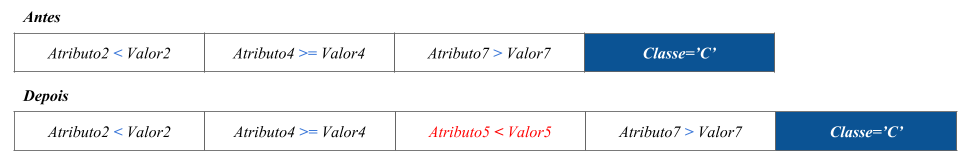
\includegraphics[scale=.5]{img/mut_1}
\caption{Exemplo de mutação por adição de novo termo na regra codificada pela partícula.}
\label{fig:mut_1}
\end{figure}

Cabe ressaltar que o mDPSO não implementa nenhum mecanismo que permita a alteração do elemento {\em atributo} para tríades do tipo \textit{<atributo, operador, valor numérico>} e do tipo \textit{<atributo, operador, outro atributo>}. Assim, este é o único operador implementado pelo mDPSO que permite a introdução de novos atributos que não foram avaliados em nenhuma partícula do enxame. Por outro lado, os elementos da tríade: ``operador'' e ``valor numérico'', podem ser perturbados (mutados) pelos mecanismos de mutação implementados no mDPSO.

\subsubsection{Mudança de Operador}
\label{sec:mdpso_mut2} 

Outro tipo de mutação implementado pelo mDPSO, ilustrado na Figura \ref{fig:mut_2}, permite a alteração de um operador lógico no termo de uma regra da partícula. Em resumo, este operador escolhe aleatoriamente um termo da regra e faz a sua substituição por outro operador segundo a distribuição de probabilidades apresentada na Tabela \ref{tab:prob_operadores}. O operador relacional modificado pelo operador ``Mudança de Operador'' está realçado na cor vermelha da Figura \ref{fig:mut_2}.

\begin{figure}[ht]
\centering
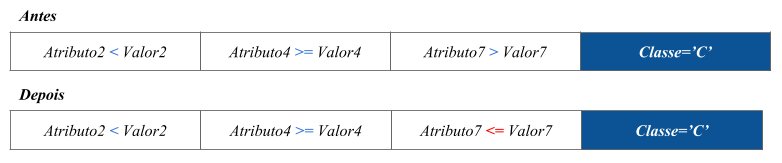
\includegraphics[scale=.5]{img/mut_2}
\caption{Exemplo de mutação por mudança de operador.}
\label{fig:mut_2}
\end{figure}

\subsubsection{Adição ou Subtração do Valor Númerico}
\label{sec:mdpso_mut3} 

Esse tipo de mutação ocorre somente quando o termo da regra apresenta  estrutura do tipo: \textit{<atributo, operador, valor numérico>}. Em resumo, este operador tem o seguinte funcionamento: (i) É selecionado aleatoriamente um termo da regra codificada na partícula; (ii) É adicionado ou subtraído um valor do terceiro elemento do termo ({valor númerico}). 

O valor da perturbação, a ser adicionado ou subtraído do elemento ``valor numérico'' no termo da regra pode ser obtido de duas formas distintas, baseado no trabalho de \citeonline{Jancauskas_2014}: (i) Valor aleatório gerado segundo uma distribuição uniforme (linha 12 do Algoritmo \ref{alg:mut}); (ii) Valor aleatório gerado segundo uma distribuição normal (gaussiana) (linha 8 do Algoritmo \ref{alg:mut}).

O funcionamento do operador de mutação proposto é ilustrado na Figura \ref{fig:mut_3}: ``NovoValor7'' refere-se ao valor resultante da adição/substração de um valor numério ao valor ``valor7'' do terceiro termo da regra.

\begin{figure}[ht]
\centering
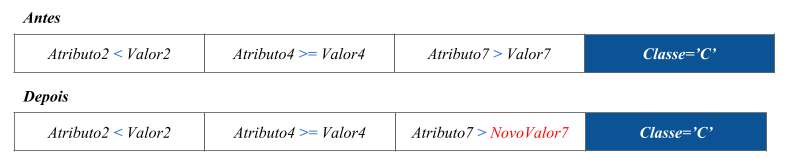
\includegraphics[scale=.5]{img/mut_3}
\caption{Exemplo de mutação por mudança de um novo valor numérico.}
\label{fig:mut_3}
\end{figure}


\subsection{Operação de Recombinação de Partículas}
\label{sec:mdpso_recomb_part}

A recombinação entre as partículas tem o objetivo de combinar características de duas partículas pais com o intuito de gerar regras mais promissoras que as originais. O mecanismo de recombinação de partículas implementado pelo mDPSO é detalhado pelo Algoritmo \ref{alg:recomb}. A variável $pl$ é uma partícula genérica, utilizada tanto para designar a partícula líder tanto em $C_k.gbest$ quanto em $p.pbest$ (Ver Algoritmo \ref{alg:mdpso_atualiza_part}), visto que ambas as recombinações são realizadas de forma similar. 

A representação proposta neste trabalho permite que partículas com tamanhos (número de termos) distintos de regras possam ser recombinadas. Diante disto, o operador de recombinação implementado pelo mDPSO retorna uma nova regra, resultante da recombinação da partícula corrente $p$ e da partícula líder em $p.pbest$ ou $C_k.gbest$, com variação do número de termos entre 1 e o valor máximo de [$|p|$, $|p.pbest|$, $|C_k.gbest|$], onde $|x|$ retorna o número de termos presentes na partícula $x$. 

Cabe mencionar que durante a operação de recombinação a partícula resultante pode apresentar um número reduzido de termos. Tal alteração no número de termos da regra durante a recombinação, deve-se à aleatoriedade do processo de seleção dos termos a serem adicionados à solução filha, bem como o mecanismo de eliminação de termos repetidos implementado pelas partículas no mDPSO.

\begin{algorithm}[ht]
\caption{Recombinação entre partículas}.
\label{alg:recomb}
\begin{algorithmic}[1]
\INPUT{$p$ - Partícula; $pl$ - Partícula líder ({\em gbest} ou {\em pbest}).}
\State $RF \leftarrow \emptyset$; // Regra Filha
\For{$k < |pl|$}
	\If{$rand < 0.5$}
		\State $RF \leftarrow$ $RF$ $\ \cup$ \{Termo aleatório da regra de $pl$\};
	\Else
		\State $RF \leftarrow$ $RF$ $\ \cup$ \{Termo aleatório da regra de $p$\};
	\EndIf
\EndFor
\For{$k < |p|$}
	\State $RF \leftarrow$ $RF$ $\ \cup$ \{Termo aleatório da regra de $p$\};
\EndFor
\State \Return $RF$;
\end{algorithmic}
\end{algorithm}

A Figura \ref{fig:recomb} ilustra o processo de recombinação entre duas regras pais e a regra filha resultante da recombinação. As setas posicionadas na parte superior de cada termo pai  indicam quais termos foram selecionados aleatoriamente para geração da regra filha.

\begin{figure}[ht]
\centering
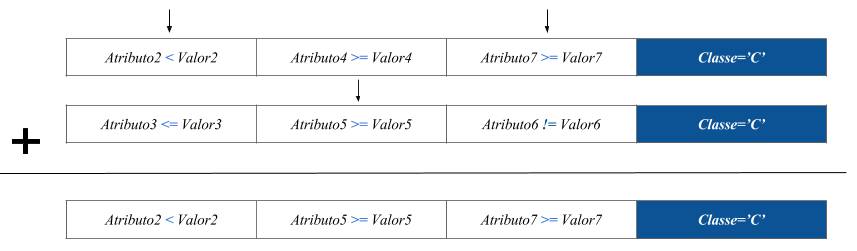
\includegraphics[scale=.5]{img/recombinacao}
\caption{Ilustração do operador de recombinação entre as partículas implementado pelo mDPSO.}
\label{fig:recomb}
\end{figure}

\section{Busca Local Pareto}
\label{sec:mdpso_busca_local}

Mecanismos de busca local são importantes por possibilitar refinamentos das soluções obtidas por um algoritmo de otimização combinatória. O Algoritmo \ref{alg:BLP} detalha o mecanismo de busca local Pareto, baseado no método {\em Neutral Improvement Pareto} (NPI) (Ver Algoritmo \ref{alg:NPI}), executado ao final de cada iteração do mDPSO com objetivo de introduzir novas soluções não-dominadas no repositório $C_k.gbest$. 

Durante a implementação da rotina de busca local Pareto proposta, observou-se que o NPI foi a abordagem que apresentou os melhores resultados quando comparado com o BFI e FPI, sendo por isso implementado pelo mDPSO. 

Além disso, um mecanismo de geração de soluções vizinhas (linha 4 do Algoritmo) baseada na mutação gaussiana é também utilizado. Esta mutação se mostrou eficiente em várias situações estudadas por \citeonline{Higashi_2003} e, para o problema analisado neste trabalho, apresentou bons resultados ao ser combinada com NPI na rotina de busca local Pareto proposta.  

Em resumo, determina-se o número máximo de $(\ceil[\big]{\log{(N)}} + 1)$ de iterações da rotina (linha 1 do Algoritmo \ref{alg:BLP}), onde $N$ refere-se ao número de atributos da base de dados. Caso seja encontrado uma solução não-dominada na vizinhança da partícula $p$, interrompe-se a rotina e atualiza-se as soluções não-dominadas do repositório $C_k.gbest$.

\begin{algorithm}[ht]
\caption{Busca Local Pareto}
\label{alg:BLP}
\begin{algorithmic}[1]
\INPUT{$p$ - Partícula; $N$ - Número de atributos da base de dados; $A$ - Conjunto de soluções não-dominadas de $C_k.gbest$;}
\State $L \leftarrow \ceil[\big]{\log{(N)}} + 1$;
\State $i \leftarrow 0$;
\While{$i < L$} 
  \State $p' \leftarrow $ Mutação($p$, gaussiana);
  \State // se a regra associada a $p'$ foi gerada anteriormente $p'.visited$
  \If{$p'.visited$ é TRUE}
    \State \textbf{continue};
  \EndIf
  \State $p'.visited \leftarrow$ TRUE;
  \State Avaliar $p'$;
  \If{$f(p') \parallel f(p) \vee f(p') \prec f(p)$} // $\parallel$ - \small{não há relação de dominância}
  	\State $C_k.gbest \leftarrow merge(C_k.gbest, \{p'\})$;
    \State $i \leftarrow L$;
  \EndIf
  \State $i \leftarrow i + 1$;
\EndWhile
\end{algorithmic}
\end{algorithm}


\section{Conclusão}

Este capítulo descreve o algoritmo biobjetivo, denominado mDPSO, baseado no algoritmo PSO para classificação de dados por meio de extração de regras. Os objetivos (efetividade e complexidade) foram considerados a fim de obter boas regras de classificação e evitar o {\em overfitting}. Outra vantagem desta abordagem é a busca por regras menores, mais fáceis de serem entendidas e interpretadas.  

Além do mais, o algoritmo proposto implementa várias funcionalidades, tais como, por exemplo, técnicas de nicho, rotina para geração da população inicial, mecanismos de recombinação e mutação específicos bem como um mecanismo de busca local Pareto. 



% ---------
% Resultados
% ---------

\chapter{Resultados Experimentais}
\label{ch:resultados}

O presente capítulo avalia o desempenho do \textbf{mDPSO} frente aos algoritmos implementados pelo WEKA: \textbf{J48} (Árvore de Decisão) \cite{Quinlan_1986},  Redes Neurais do tipo Função de Base Radial (\textbf{RBF}, {\em Radial Basis Function}) \cite{Broomhead_1988} e o \textbf{SMO} ({\em Sequential Minimal Optimization}) \cite{Keerthi_2001}, uma variante da Máquina de Vetores de Suporte (SVM, {\em Support Vector Machine}) em 07 (sete) bases de dados selecionadas para testes.

\section{Introdução}

O mDPSO foi implementado utilizando a linguagem {\em Java} 1.8 64-bits integrado com o banco de dados {\em PostgreSQL} 9.1 para armazenamento e manipulação das base de dados utilizadas. Os testes foram realizados em um PC Intel (R) Core (TM) i3-4330 CPU 3.50G Hz com 8.00GB de memória RAM e sistema operacional {\em Windows 10} 64-bits.

A metodologia de análise dos resultados é similar à utilizada por \citeonline{Pereira_2012}. Os seguintes algoritmos J48, RBF e SMO foram implementados pelo {\em software} WEKA e avaliados considerando somente o produto da sensibilidade pela especificidade global. Este cálculo é realizado da seguinte forma: se determinado algoritmo para a base {\em Wine} obteve os seguintes resultados: $0.93$ para classe A; $0.90$ para B e $0.99$ para classe C, o produto da sensibilidade pela especificidade global é calculado como a média dos desempenhos nas três classes: $(0.93+0.90+0.99)/3 = 0.94$. 

O mDPSO, por sua vez, realiza o mesmo cálculo utilizando a melhor regra de cada classe (nicho), baseada no valor do primeiro objetivo $f_1(I,X)$ (Ver Eq. \ref{eq:fitness1}). Dessa forma, em uma base de dados composta por três classes, o mDPSO determina três classificadores distintos, um para cada classe. Como afirma \citeonline{Handl_2007}, espera-se que os resultados gerados pelos algoritmos multiobjetivo sejam tão bons (ou melhores) do que aqueles gerados por algoritmos mono-objetivo. No caso específico deste trabalho, é esperado que os resultados gerados pelo mDPSO sejam comparáveis com os resultados obtidos com os  algoritmos estudados, implementados pelo WEKA.

Foram avaliados os desempenhos de 04 (quatro) algoritmos (mDPSO, J48, SMO e RBF) para 07 (sete) bases de dados, caracterizadas a seguir: 

\begin{itemize}
	\item \textbf{Diabetes}: Possui 8 atributos numéricos  e 768 instâncias alocadas em duas classes: \emph{tested positive} (500) e \emph{tested negative} (268);
 
	\item \textbf{DGA 1}: Possui 5 atributos numéricos e 149 instâncias divididas em três classes: {\em Normal} (84), {\em Falha Elétrica} (62) e {\em Falha Térmica} (78).
	
	\item \textbf{DGA 2}: Possui 5 atributos numéricos e 224 instâncias divididas em três classes: {\em Normal} (122), {\em Falha Elétrica} (10) e {\em Falha Térmica} (17).
 
	\item \textbf{Hepatitis}: Possui 19 atributos numéricos e 155 instâncias distribuídas em duas classes: \emph{to die} (32) e \emph{to live} (123); 
 
	\item \textbf{Ionosphere}: Possui 30 atributos numéricos e 351 instâncias distribuídas nas classes: \emph{good} (225) e \emph{bad} (126);
 
	\item \textbf{Unbalanced}: Possui 32 atributos numéricos e 856 instâncias distribuídas em duas classes: \emph{active} (12) e \emph{inactive} (844).
  
	\item \textbf{Wine}: Possui 13 atributos numéricos e 178 instâncias divididas em três classes: A (59), B (71) e C (48);
\end{itemize}

Sendo que as bases de dados {\em DG1}, {\em DG2}, {\em Hepatitis} e {\em Wine} foram as mesmas analisadas no trabalho de \citeonline{Pereira_2014}.

Durante a avaliação do desempenho dos algoritmos utilizou-se a {\em validação cruzada k=10-fold} (10 partições) que consiste em dividir a base de dados em {\em k} subconjuntos, sendo {\em k-1} partições para treinamento e 01 (uma) para teste. Este processo de treinamento e teste é repetido com todos os {\em k} subconjuntos e a média dos resultados obtido é utilizada como indicador da qualidade do modelo \cite{Castro_2016}.

A validação cruzada utilizada é estratificada e consiste em distribuir uniformemente as classes das amostras entre as partições. Por exemplo, dado um conjunto de dados dividido em duas classes e sabendo que a {\em classe A} possui 20\% dos objetos e a {\em classe B} possui 80\% das amostras. Ao se fazer a separação da base de treinamento e teste é garantido a manutenção da mesma proporção entre as {\em k} partições. Para os testes realizados, as mesmas partições são utilizadas em todos os algoritmos de maneira a tentar prover uma justa comparação entre os algoritmos analisados. 

Com objetivo de atestar o desempenho dos algoritmos: mDPSO, J48, SMO e RBF, segundo o produto da sensibilidade pela especificidade global, foram aplicados os seguintes testes estatísticos: Teste {\em Kolgomorov-Smirnov} para verificação da normalidades das amostras; teste {\em One-Way Analysis of Variance} (ANOVA) e o teste {\em post-hoc Tukey} para construção de um {\em ranking} de desempenho dos algoritmos - O {\em ranking} pode indicar performance superior, similar (empate) ou inferior entre os algoritmos. É importante frisar que os testes devem ser realizados na ordem apresentada.

Para realização dos testes  {\em post-hoc Tukey}, adotou-se o valor de confiança igual a 95\% (o mesmo adotado no trabalho de \citeonline{Pereira_2012}). Logo, se o p-valor retornado pelo teste for inferior a $0.05$, sugere-se que o desempenho do par de algoritmos analisados é estatisticamente diferente. Do contrário, não há diferença estatística significativa entre ambos. Dessa maneira, se o desempenho de ambos algoritmos não apresentarem diferenças significativas entre eles, então ambos são alocados na mesma posição do {\em ranking}. 

Segundo \citeonline{Carrano_2011}, a avaliação de desempenho de algoritmos não-determinísticos, tais como Algoritmos Evolutivos, não pode ser realizada utilizando resultados de algoritmos determinísticos para cada instância do problema. A natureza estocástica desses métodos introduz uma variabilidade aleatória na resposta fornecida pelo algoritmo, uma vez que a solução obtida pelo mesmo pode variar consideravelmente a cada execução. Ainda que a mesma solução seja obtida, o tempo computacional necessário para alcançar tal solução é geralmente diferente em diferentes execuções do mesmo algoritmo.

\section{Parâmetros dos Algoritmos}

Para o mDPSO, os parâmetros $\omega$, $c_1$ e $c_2$ foram definidas com os seguintes valores de 0.9, 0.8 e 0.8 respectivamente, sendo tais valores escolhidos por meio de experimentações. Foram utilizadas 90 partículas com critério de parada de 30000 avaliações da função-objetivo em todas as bases de dados analisadas neste trabalho.

Os parâmetros utilizados pelos 03 (três) algoritmos implementados pela ferramenta WEKA, para cada base de dados, são listados na Tabela \ref{tab:config_weka}. A escolha destes parâmetros foi inspirada no trabalho de \citeonline{Pereira_2014}, sendo utilizadas as melhores configurações obtidas por meio de experimentações durante o desenvolvimento deste trabalho:

\begin{table}[ht]
\setlength{\arrayrulewidth}{.2em}
\vspace{12pt}
\centering{}
\scalebox{0.6}{
\begin{tabular}{ l l l l l l l l l }
	\hline \textbf{Algoritmo} & \textbf{Parâmetros} & \textbf{Diabe.} & \textbf{DGA 1} & \textbf{DGA 2} & \textbf{Hepat.} & \textbf{Ionos.} & \textbf{Unbal.} & \textbf{Wine}   \\
  \hline 
  \textbf{J48} & {\em Pruned}                     & Sim        & Sim        & Sim        & Sim        & Sim        & Sim        & Sim  \\
               & {\em Confidence factor}          & 0.25       & 0.025      & 0.25       & 0.025      & 0.25       & 0.25       & 0.25 \\
  \textbf{SMO} & {\em Complexity parameter C}     & 2.0        & 3.0        & 4.0        & 1.0        & 2.0        & 2.0        & 2.0  \\
               & {\em Kernel function}            & PolyKernel & PolyKernel & PolyKernel & PolyKernel & PolyKernel & PolyKernel & PolyKernel \\
               & {\em Function exponent}          & 2.0        & 3.0        & 1.0        & 2.0        & 2.0        & 2.0        & 2.0  \\  
  \textbf{RBF} & {\em Clusters}                   & 3          & 2          & 4          & 3          & 3          & 3          & 3    \\
               & {\em Min. std. dev. clusters}    & 0.1        & 0.01       & 0.01       & 0.1        & 0.1        & 0.1        & 0.1  \\
 \hline
\end{tabular}
}
\caption{Parâmetros de configuração do WEKA em cada base de dados.}
\label{tab:config_weka}
\end{table}

\section{Análise Baseada na Métrica Sensibilidade $\times$ Especificidade Global}
\label{sec:mdpso_analise2}

Nesta seção do trabalho, faz-se a descrição dos resultados obtidos com cada algoritmo utilizando a métrica sensibilidade $\times$ especificidade para cada base de dados. Nesta fase do trabalho, somente serão avaliados os resultados gerados pelos algoritmos mDPSO e os algoritmos implementados no WEKA. 

O produto da sensibilidade pela especificidade global relativo às 50 execuções (amostras) de cada algoritmo, na base de dados {\em Diabetes}, é apresentado na Figura \ref{fig:diabetes}. Os resultados apresentados pelo gráfico mostram que o mDPSO apresentou o melhor desempenho para a base {\em Diabetes}, com média superior aos demais. Observa-se também que os valores médios obtidos para a métrica sensibilidade $\times$ especificidade entre os algoritmos J48 e SMO ficaram bem próximos, com uma pequena vantagem para o SMO. Observa-se também ue o desvio padrão obtido pelo j48 é superior ao obtido pelo SMO. O RBF foi o algoritmo que apresentou o pior desempenho.

\begin{figure}[!ht]
\centering
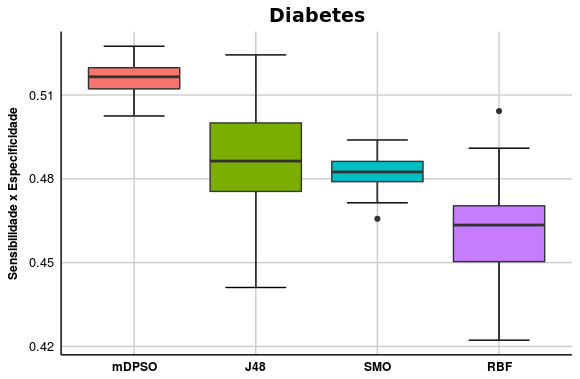
\includegraphics[scale=.7]{graficos/diabetes}
\caption{Desempenho dos algoritmos na base de dados {\em Diabetes} utilizando a métrica sensibilidade $\times$ especificidade global.}
\label{fig:diabetes}
\end{figure}

Para todas as bases de dados analisadas, o p-valor obtido pelo teste ANOVA (com valor de confiança adotado de 95\%) foi de aproximadamente 0 (zero). Deste modo, a Tabela \ref{tab:pvalor_diabetes} apresenta a relação entre os pares de algoritmos de acordo com o p-valor obtido pelo teste {\em Tukey} para a base {\em Diabetes}. Os resultados mostram que não houveram diferenças significativas do desempenho pelo produto da sensibilidade pela especificidade global para as 50 execuções entre os algoritmos J48 e SMO, o que sugere que ambos os algoritmos J48 e SMO apresentaram desempenho similar para esta base de dados. O mDPSO não apresentou diferenças significativas em relação a todos algoritmos implementados pelo WEKA. 

\begin{table}[!ht]
\setlength{\arrayrulewidth}{.2em}
\vspace{12pt}
\centering{}
\scalebox{0.8}{
\begin{tabular}{ c c c c c}
  \hline           & \textbf{mDPSO} & \textbf{J48}   & \textbf{SMO}   & \textbf{RBF} \\
  \hline 
    \textbf{mDPSO} &              - &         0.0000 &         0.0000 &       0.0000 \\
    \textbf{J48}   &         0.0000 &              - &         0.2804 &       0.0000 \\
    \textbf{SMO}   &         0.0000 &         0.2804 &              - &       0.0000 \\
    \textbf{RBF}   &         0.0000 &         0.0000 &         0.0000 &            - \\
  \hline
\end{tabular}
}
\caption{p-valor medido para o produto da sensibilidade pela especificidade global de cada algoritmo na base de dados {\em Diabetes}.}
\label{tab:pvalor_diabetes}
\end{table}

De forma semelhante, analisou-se o desempenho dos algoritmos nas demais bases de dados. As Figuras \ref{fig:dga_1} e \ref{fig:dga_2} ilustram o desempenho de cada algoritmo para as bases {\em DGA 1} e {\em DGA 2} respectivamente. Percebe-se que em ambas as bases de dados, o mDPSO gerou resultados superiores aos demais algoritmos. Também nota-se que os resultados gerados pelo SMO foram os que mais se aproximaram dos resultados do mDPSO na base {\em DGA 1}. Ainda nesta base, o pior desempenho foi o do algoritmo J48. E na base {\em DGA 2}, os resultados gerados pelo mDPSO foram bem superiores aos dos demais algoritmos. Por outro lado, o algoritmo SMO apresentou o pior desempenho nesta base que se caracteriza por ser bastante desbalanceada. 

\begin{figure}[!ht]
\centering
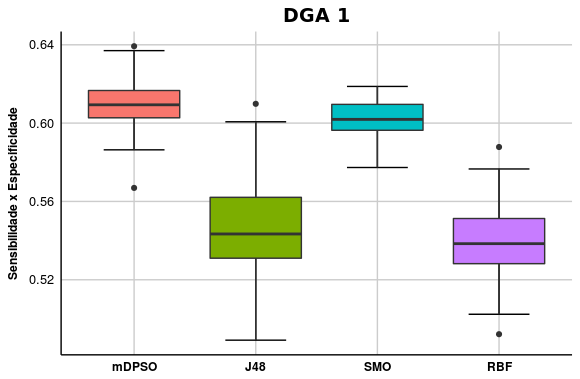
\includegraphics[scale=.7]{graficos/DGA1}
\caption{Desempenho de cada algoritmo na base de dados {\em DGA 1} utilizando a métrica sensibilidade $\times$ especificidade global.}
\label{fig:dga_1}
\end{figure}

A Tabela \ref{tab:pvalor_dga1} apresenta a relação entre os pares de algoritmos de acordo com o p-valor obtido do teste {\em Tukey} para a base {\em DGA 1}. Observa-se que apesar do desempenho superior do mDPSO, não houveram diferenças significativas entre os desempenhos dos algoritmos mDPSO e SMO. O mesmo comportamento foi observado entre os algoritmos J48 e RBF, ficando estes abaixo do desempenho obtido pelo algoritmos mDPSO e SMO.

\begin{table}[!ht]
\setlength{\arrayrulewidth}{.2em}
\vspace{12pt}
\centering{}
\scalebox{0.8}{
\begin{tabular}{ c c c c c}
  \hline           & \textbf{mDPSO} & \textbf{J48}   & \textbf{SMO}   & \textbf{RBF} \\
  \hline 
    \textbf{mDPSO} &              - &         0.0000 &         0.0684 &       0.0000 \\
    \textbf{J48}   &         0.0000 &              - &         0.0000 &       0.0938 \\
    \textbf{SMO}   &         0.0684 &         0.0000 &              - &       0.0000 \\
    \textbf{RBF}   &         0.0000 &         0.0938 &         0.0000 &            - \\
  \hline
\end{tabular}
}
\caption{p-valor medido para o produto da sensibilidade pela especificidade global de cada algoritmo na base de dados {\em DGA 1}.}
\label{tab:pvalor_dga1}
\end{table}

\begin{figure}[!ht]
\centering
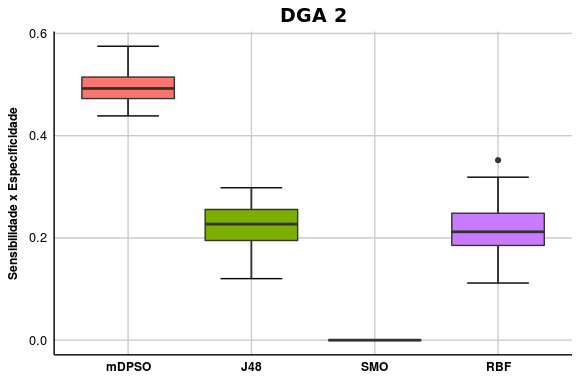
\includegraphics[scale=.7]{graficos/DGA2}
\caption{Desempenho de cada algoritmo na base de dados {\em DGA 2} utilizando a métrica sensibilidade $\times$ especificidade global.}
\label{fig:dga_2}
\end{figure}

Na Tabela \ref{tab:pvalor_dga2} é apresentada a relação entre os pares de algoritmos de acordo com o p-valor obtido para a base {\em DGA 2}. Os resultados apresentados mostram que os valores gerados pelos algoritmos mDPSO são distintos dos demais algoritmos. Os resultados também sinalizam que não se pode afirmar que o algoritmo J48 possui desempenho superior ao desempenho do RBF. Diferentemente da base {\em DGA 1}, o SMO foi o que apresentou o pior desempenho, isso possivelmente devido ao grau de desabalanceamento da base {\em DGA 2} em comparação a base {\em DG1}.

\begin{table}[!ht]
\setlength{\arrayrulewidth}{.2em}
\vspace{12pt}
\centering{}
\scalebox{0.8}{
\begin{tabular}{ c c c c c}
  \hline           & \textbf{mDPSO} & \textbf{J48}   & \textbf{SMO}   & \textbf{RBF} \\
  \hline 
    \textbf{mDPSO} &              - &         0.0000 &         0.0000 &       0.0000 \\
    \textbf{J48}   &         0.0000 &              - &         0.0000 &       0.8481 \\
    \textbf{SMO}   &         0.0000 &         0.0000 &              - &       0.0000 \\
    \textbf{RBF}   &         0.0000 &         0.8481 &         0.0000 &            - \\
  \hline
\end{tabular}
}
\caption{p-valor medido para o produto da sensibilidade $\times$ especificidade global de cada algoritmo na base de dados {\em DGA 2} global.}
\label{tab:pvalor_dga2}
\end{table}

Para a base {\em Hepatitis}, o gráfico da Figura \ref{fig:hepatitis} mostra o bom desempenho dos algoritmos RBF, mDPSO e SMO, sendo possível perceber o desempenho considerado superior do algoritmo RBF. Durante a avaliação entre os pares de algoritmos segundo os p-valores obtidos para esta base e conforme apresentados na Tabela \ref{tab:pvalor_hepatitis}, revelam que não houveram diferenças estatísticas significativas entre o mDPSO e o SMO, constatando o desempenho superior do RBF. O algoritmo J48 foi o que apresentou o pior desempenho.

\begin{figure}[!ht]
\centering
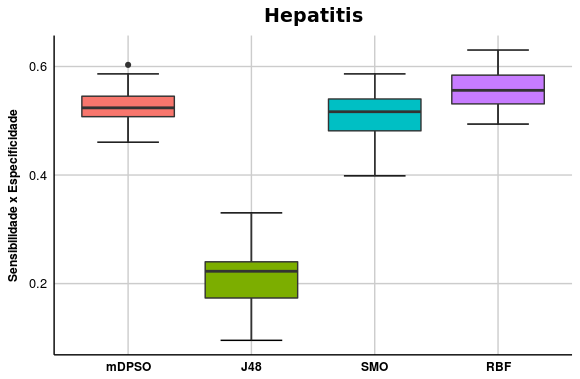
\includegraphics[scale=.7]{graficos/hepatitis}
\caption{Desempenho de cada algoritmo na base de dados {\em Hepatitis} utilizando a métrica sensibilidade $\times$ especificidade global.}
\label{fig:hepatitis}
\end{figure}

\begin{table}[!ht]
\setlength{\arrayrulewidth}{.2em}
\vspace{12pt}
\centering{}
\scalebox{0.8}{
\begin{tabular}{ c c c c c}
  \hline           & \textbf{mDPSO} & \textbf{J48}   & \textbf{SMO}   & \textbf{RBF} \\
  \hline 
    \textbf{mDPSO} &              - &         0.0000 &         0.1767 &       0.0028 \\
    \textbf{J48}   &         0.0000 &              - &         0.0000 &       0.0000 \\
    \textbf{SMO}   &         0.1767 &         0.0000 &              - &       0.0000 \\
    \textbf{RBF}   &         0.0028 &         0.0000 &         0.0000 &            - \\
  \hline
\end{tabular}
}
\caption{p-valor medido para o produto da sensibilidade pela especificidade global de cada algoritmo na base de dados {\em Hepatitis}.}
\label{tab:pvalor_hepatitis}
\end{table}

Testes na base {\em Ionosphere} mostraram o desempenho ruim do mDPSO frente aos demais algoritmos implementados pelo WEKA. Além disso, como mostrado na Figura \ref{fig:ionosphere}, percebe-se com certa facilidade que o algoritmo RBF apresentou desempenho superior em relação às outras implementações. Ademais, de acordo com a Tabela \ref{tab:pvalor_ionosphere} os algoritmos apresentaram diferenças estatísticas significativas entre si, caracterizando desempenhos diferenciados entre os algoritmos para esta base de dados.

\begin{figure}[!ht]
\centering
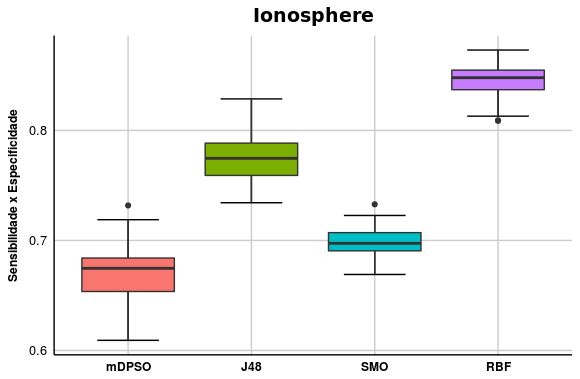
\includegraphics[scale=.7]{graficos/ionosphere}
\caption{Desempenho de cada algoritmo na base de dados {\em Ionosphere} utilizando a métrica sensibilidade $\times$ especificidade global.}
\label{fig:ionosphere}
\end{figure}

\begin{table}[!ht]
\setlength{\arrayrulewidth}{.2em}
\vspace{12pt}
\centering{}
\scalebox{0.8}{
\begin{tabular}{ c c c c c}
  \hline           & \textbf{mDPSO} & \textbf{J48}   & \textbf{SMO}   & \textbf{RBF} \\
  \hline 
    \textbf{mDPSO} &              - &         0.0000 &         0.0000 &       0.0000 \\
    \textbf{J48}   &         0.0000 &              - &         0.0000 &       0.0000 \\
    \textbf{SMO}   &         0.0000 &         0.0000 &              - &       0.0000 \\
    \textbf{RBF}   &         0.0000 &         0.0000 &         0.0000 &            - \\
  \hline
\end{tabular}
}
\caption{p-valor medido para o produto da sensibilidade pela especificidade global de cada algoritmo na base de dados {\em Ionosphere}.}
\label{tab:pvalor_ionosphere}
\end{table}

Diante do baixo desempenho do algoritmo mDPSO na base \emph{Ionosphere}, analisou-se o produto da sensibilidade pela especificidade de cada classe  (classes {\em good} e {\em bad}) desta base para cada algoritmo. Os resultados obtidos, listados na Tabela \ref{tab:sen_esp_classe_ionosphere},  mostram que, apesar do mDPSO obter um bom desempenho para a classe {\em good}, os resultados obtidos para a classe {\em bad} influenciam negativamente o desempenho geral do algoritmo. É importante comentar que os resultados semelhantes gerados pelos algoritmos J48, SMO e RBF devem-se ao cálculo do produto da especificidade pela sensibilidade em bases binárias (com duas classes). Como o mDPSO utiliza técnicas de nicho e são escolhidas as melhores regras de cada nicho, consequentemente, cada classe (nicho) possui um classificador distinto com desempenhos diferentes. 

\begin{table}[!ht]
\setlength{\arrayrulewidth}{.2em}
\vspace{12pt}
\centering{}
\scalebox{0.8}{
\begin{tabular}{ l l l l }
  \hline         & \textbf{bad}             & \textbf{good}        \\
  \hline  
  \textbf{mDPSO} &         0.5081 (0.0406)  &         0.8340 (0.0208)  \\
  \textbf{J48}   &         0.7752 (0.0229)  &         0.7752 (0.0229)  \\
  \textbf{SMO}   &         0.6988 (0.0132)  &         0.6988 (0.0132)  \\
  \textbf{RBF}   & \textbf{0.8451 (0.0145)} & \textbf{0.8451 (0.0145)} \\
  \hline
\end{tabular}
}
\caption{Desempenho de cada algoritmo usando o produto da sensibilidade pela especificidade em cada classe na base {\em Ionosphere} global.}
\label{tab:sen_esp_classe_ionosphere}
\end{table}

Para o conjunto de bases analisadas neste trabalho, a base {\em Unbalanced} caracteriza-se como a mais desabalanceada. E novamente, tal como ocorre na base {\em DGA 2}, o mDPSO apresentou resultados superiores em relação aos demais algoritmos. Possivelmente, o desempenho ruim destes algoritmos deve-se ao fato do alto grau de desbalanceamento deste base de dados, uma vez que mostram que eles não foram capazes de identificar as duas classes da base, sendo penalizados quando avaliado o produto da sensibilidade pela especificidade.

\begin{figure}[!ht]
\centering
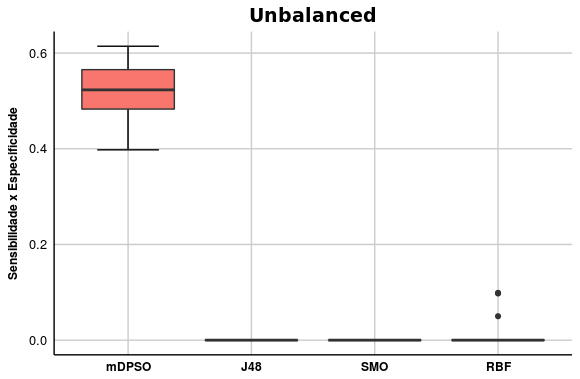
\includegraphics[scale=.7]{graficos/unbalanced}
\caption{Desempenho de cada algoritmo na base de dados {\em Unbalanced} utilizando a métrica sensibilidade $\times$ especificidade global.}
\label{fig:unbalanced}
\end{figure}

Na Tabela \ref{tab:pvalor_unbalanced} é apresentada a relação entre os pares de algoritmos de acordo com o p-valor obtido para a base {\em Unbalanced}. Os dados mostram que os resultados do mDPSO não possuem nenhuma similaridade com os dos outros três algoritmos. 

\begin{table}[!ht]
\setlength{\arrayrulewidth}{.2em}
\vspace{12pt}
\centering{}
\scalebox{0.8}{
\begin{tabular}{ c c c c c}
  \hline           & \textbf{mDPSO} & \textbf{J48}   & \textbf{SMO}   & \textbf{RBF} \\
  \hline 
    \textbf{mDPSO} &              - &         0.0000 &         0.0000 &       0.0000 \\
    \textbf{J48}   &         0.0000 &              - &         1.0000 &       0.8599 \\
    \textbf{SMO}   &         0.0000 &         1.0000 &              - &       0.8599 \\
    \textbf{RBF}   &         0.0000 &         0.8599 &         0.8599 &            - \\
  \hline
\end{tabular}
}
\caption{p-valor medido para o produto da sensibilidade pela especificidade global de cada algoritmo na base de dados {\em Unbalanced}.}
\label{tab:pvalor_unbalanced}
\end{table}

Por fim, a Figura \ref{fig:wine} mostra o gráfico de desempenho dos algoritmos para a base {\em Wine}, segundo os valores obtidos para a métrica sensibilidade $\times$ especificidade global. A figura ilustra o bom desempenho dos algoritmos SMO e RBF frente aos outros dois (mDPSO e J48).  

Além disso, ao avaliar os pares de algoritmos segundo o p-valor computado para a base {\em Wine}, conforme descrito na Tabela \ref{tab:pvalor_wine}, verifica-se que não houveram diferenças estatísticas significativa entre os algoritmos SMO e o RBF. Novamente, o J48 apresentou o pior desempenho. Para esta base, o mDPSO obteve desempenho considerado intermediário, com diferenças estatísticas de desempenho entre os demais algoritmos implementados pelo WEKA.

\begin{figure}[!ht]
\centering
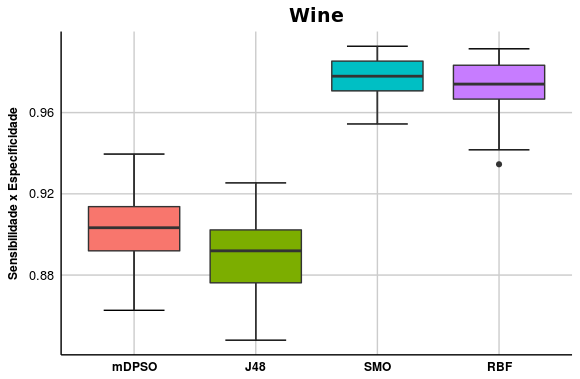
\includegraphics[scale=.7]{graficos/wine}
\caption{Desempenho de cada algoritmo na base de dados {\em Wine} utilizando a métrica sensibilidade $\times$ especificidade global.}
\label{fig:wine}
\end{figure}

\begin{table}[!ht]
\setlength{\arrayrulewidth}{.2em}
\vspace{12pt}
\centering{}
\scalebox{0.8}{
\begin{tabular}{ c c c c c}
  \hline           & \textbf{mDPSO} & \textbf{J48}   & \textbf{SMO}   & \textbf{RBF} \\
  \hline 
    \textbf{mDPSO} &              - &         0.0617 &         0.0000 &       0.0000 \\
    \textbf{J48}   &         0.0617 &              - &         0.0000 &       0.0000 \\
    \textbf{SMO}   &         0.0000 &         0.0000 &              - &       0.4286 \\
    \textbf{RBF}   &         0.0000 &         0.0000 &         0.4286 &            - \\
  \hline
\end{tabular}
}
\caption{p-valor medido para o produto da sensibilidade $\times$ especificidade global de cada algoritmo na base de dados {\em Wine}.}
\label{tab:pvalor_wine}
\end{table}

Mais uma vez, motivado pelo desempenho ruim do mDPSO na base \emph{Wine}, investigou-se o desempenho dos algoritmos para cada classe desta base. Os resultados obtidos são exibidos na Tabela \ref{tab:sen_esp_classe_wine}. Um aspecto que chama a atenção em relação a base {\em Wine} é que o mDPSO apresenta um desempenho ruim por classe, especialmente para a classe B, na qual apresentou o pior desempenho entre os algoritmos analisados, influenciando negativamente no desempenho do mDPSO. 

\begin{table}[!ht]
\setlength{\arrayrulewidth}{.2em}
\vspace{12pt}
\centering{}
\scalebox{0.7}{
\begin{tabular}{ l l l l l}
  \hline         & \textbf{Classe A}        & \textbf{Classe B}        & \textbf{Classe C}            \\
  \hline  
  \textbf{mDPSO} &         0.9487 (0.0190)  &         0.8178 (0.0357)  &         0.9426 (0.0229)  \\
  \textbf{J48}   &         0.9255 (0.0223)  &         0.8662 (0.0228)  &         0.8825 (0.0254)  \\
  \textbf{SMO}   & \textbf{0.9937 (0.0091)} &         0.9580 (0.0155)  &         0.9787 (0.0109)  \\
  \textbf{RBF}   &         0.9643 (0.0142)  & \textbf{0.9664 (0.0164)} & \textbf{0.9889 (0.0131)} \\
  \hline
\end{tabular}
}
\caption{Desempenho dos algoritmos segundo a métrica sensibilidade $\times$ especificidade para cada classe da base {\em Wine}.}
\label{tab:sen_esp_classe_wine}
\end{table}

Finalmente, na Tabela \ref{tab:sen_esp_global} é apresentada a média (desvio padrão) das 50 execuções do produto da sensibilidade pela especificidade global dos 05 (cinco) algoritmos para as 07 (sete) bases de dados analisadas neste trabalho. Observa-se que apesar do desempenho ruim nas bases {\em Ionosphere} e {\em Wine}, o mDPSO conseguiu resultados considerados bons nas demais bases de dados. Particularmente, para as bases de dados {\em Diabetes}, {\em DGA 1} e {\em Unbalanced}, em que apresentou os melhores indicadores de desempenho. Além do mais, apesar do bom desempenho do algoritmo PG na base {\em DGA 2}, o desvio padrão calculado para este algoritmo é superior (aproximadamente 435\%) ao desvio computado para o mDPSO, o que mostra o bom desempenho deste algoritmo para esta base. Para facilitar a compreensão dos dados da tabela, negritou-se os melhores resultados obtidos para cada base de dados.

\begin{table}[!ht]
\setlength{\arrayrulewidth}{.2em}
\vspace{12pt}
\centering{}
\scalebox{0.6}{
\begin{tabular}{ l l l l l l l l }
  \hline           & \textbf{Diabe.}          & \textbf{DGA 1}           & \textbf{DGA 2}           & \textbf{Hepat.}          & \textbf{Ionos.}          & \textbf{Unbal.}          & \textbf{Wine}            \\
  \hline 
    \textbf{mDPSO} & \textbf{0.5159 (0.0054)} & \textbf{0.6095 (0.0121)} &         0.4935 (0.0304)  &         0.5275 (0.0336)  &         0.6710 (0.0230)  & \textbf{0.5171 (0.0591)} &         0.9030 (0.0151)  \\
    \textbf{J48}   &         0.4873 (0.0198)  &         0.5471 (0.0237)  &         0.2240 (0.0402)  &         0.2106 (0.0501)  &         0.7752 (0.0229)  &         0.0000 (0.0000)  &         0.8914 (0.0180)  \\
    \textbf{SMO}   &         0.4825 (0.0058)  &         0.6010 (0.0104)  &         0.0000 (0.0000)  &         0.5107 (0.0423)  &         0.6988 (0.0132)  &         0.0000 (0.0000)  & \textbf{0.9768 (0.0092)} \\
    \textbf{RBF}   &         0.4613 (0.0160)  &         0.5390 (0.0194)  &         0.2182 (0.0491)  & \textbf{0.5564 (0.0356)} & \textbf{0.8451 (0.0145)} &         0.0049 (0.0204)  &         0.9732 (0.0124)  \\ 
    \textbf{PG}*   &         -                &         0.5725 (0.1139)  & \textbf{0.5409 (0.1325)} &         0.5053 (0.2746)  &         -                &         -                &         0.9634 (0.0422)  \\
  \hline
\end{tabular}
}
\caption{Desempenho de cada algoritmo segundo o produto da sensibilidade pela especificidade global para cada base de dados.}
\label{tab:sen_esp_global}
\end{table}

A Tabela \ref{tab:rank_efet} apresenta o {\em ranking} de desempenho dos 04 (quatro) algoritmos para cada base de dados, de acordo estratégia similar à utilizada no trabalho de \citeonline{Pereira_2012}. Ao analisar os resultados exibidos na Tabela \ref{tab:rank_efet}, observa-se o desempenho considerado satisfatório do algoritmo mDPSO para classificação de dados nas várias bases de dados selecionadas. Em resumo, o mDPSO obteve o melhor desempenho em 04 (quatro) das 07 (sete) bases avaliadas ({\em Diabetes}, {\em DGA 1}, {\em DGA 2} e {\em Unbalanced}). Para a base de dados {\em DGA 1} o mDPSO obteve desempenho similar ao algoritmo SMO e superior aos algoritmos J48 e o RBF. Atenta-se também para o desempenho considerado ruim apresentado pelo algoritmo J48 que não conseguiu se sobressair em nenhuma das bases de dados analisadas, geralmente ocupando posições intermediárias. 

%\begin{table}[ht]
%\setlength{\arrayrulewidth}{.2em}
%\vspace{12pt}
%\centering{}
%\scalebox{0.9}{
%\begin{tabular}{ l c c c c c c c }
%	\hline & \textbf{Diabe.} & \textbf{DGA 1} & \textbf{DGA 2} & \textbf{Hepat.} & \textbf{Ionos.} & \textbf{Unbal.} & \textbf{Wine} \\
%	\hline
%    \textbf{mDPSO}   & $1^{\circ}$ & $1^{\circ}$ & $1^{\circ}$ & $2^{\circ}$ & $4^{\circ}$ & $1^{\circ}$ & $2^{\circ}$ \\
%    \textbf{J48}     & $2^{\circ}$ & $2^{\circ}$ & $2^{\circ}$ & $3^{\circ}$ & $2^{\circ}$ & $2^{\circ}$ & $3^{\circ}$ \\
%    \textbf{SMO}     & $2^{\circ}$ & $1^{\circ}$ & $3^{\circ}$ & $2^{\circ}$ & $3^{\circ}$ & $2^{\circ}$ & $1^{\circ}$ \\
%    \textbf{RBF}     & $3^{\circ}$ & $2^{\circ}$ & $2^{\circ}$ & $1^{\circ}$ & $1^{\circ}$ & $2^{\circ}$ & $1^{\circ}$ \\
% 	\hline
%\end{tabular}
%}
%\caption{{\em Ranking} de desempenho de cada algoritmo.}
%\label{tab:rank_efet}
%\end{table}

\begin{table}[ht]
\setlength{\arrayrulewidth}{.2em}
\vspace{12pt}
\centering{}
\scalebox{0.9}{
\begin{tabular}{ l c c c c c c c }
	\hline & \textbf{Diabe.} & \textbf{DGA 1} & \textbf{DGA 2} & \textbf{Hepat.} & \textbf{Ionos.} & \textbf{Unbal.} & \textbf{Wine} \\
	\hline
    \textbf{mDPSO}   & \textbf{A} & \textbf{A} & \textbf{A} & \textbf{B} & \textbf{D} & \textbf{A} & \textbf{B} \\
    \textbf{J48}     & \textbf{B} & \textbf{B} & \textbf{B} & \textbf{C} & \textbf{B} & \textbf{B} & \textbf{C} \\
    \textbf{SMO}     & \textbf{B} & \textbf{A} & \textbf{C} & \textbf{B} & \textbf{C} & \textbf{B} & \textbf{A} \\
    \textbf{RBF}     & \textbf{C} & \textbf{B} & \textbf{B} & \textbf{A} & \textbf{A} & \textbf{B} & \textbf{A} \\
 	\hline
\end{tabular}
}
\caption{{\em Ranking} de desempenho de cada algoritmo.}
\label{tab:rank_efet}
\end{table}

Cabe ressaltar que apesar de constar desempenho do algoritmo PG para algumas bases de dados não foi possível analisá-lo para inclusão no {\em ranking} de desempenho. 

Assim, de maneira geral, foi possível observar que o mDPSO apresentou resultados considerados positivos, mostrando-se competitivo quando comparado à outros métodos clássicos encontrados na literatura especializada, sendo importante destacar também o bom desempenho obtido pelo mesmo em relação às bases de dados desbalanceadas quando comparado aos demais métodos analisados implementados pelo WEKA.

\section{Conclusão}

Neste capítulo foram apresentados os resultados obtidos na comparação do algoritmo mDPSO com 03 (três) algoritmos clássicos (Árvore de Decisão, RBF e SVM) implementados pelo WEKA em 07 (sete) bases de dados previamente selecionadas. 

Os experimentos mostraram um desempenho satisfatório do algoritmo mDPSO frente aos outros 03 algoritmos avaliados neste trabalho. Os resultados revelam que o mDPSO se mostrou promissor, principalmente ao se analisar o seu desempenho em bases de dados desbalanceadas. Em relação às demais bases de dados, mostrou-se competitivo com resultados comparáveis com a Árvore de Decisão, RBF e SVM implementadas pelo WEKA em várias bases de dados analisadas no decorrer dos experimentos analisados.

% ---------
% Conclusão
% ---------
\chapter[Considerações Finais]{Considerações finais}
\label{ch:cons_finais}

A classificação de dados é um problema importante dentro da área de mineração de dados. Neste contexto, o presente trabalho teve por objetivo propor uma abordagem multiobjetivo baseada em PSO para classificação de dados por meio de extração de regras. 

Denominado de mDPSO, o algoritmo foi comparada com três métodos clássicos, reconhecidos na literatura e implementados pela ferramenta de mineração de dados WEKA, em 07 (sete) bases de dados selecionadas para testes. 

A partir dos resultados obtidos, observou-se que o mDPSO se mostrou competitivo, com desempenho considerado promissor, principalmente em bases de dados desbalanceadas, como apresentado durante a análise dos experimentos desenvolvidos neste trabalho.

O algoritmo proposto implementou as seguinte funcionalidades: geração da população inicial; um mecanismo de busca local Pareto, adaptado do NPI, para refinamento das soluções encontradas; e operadores de recombinação e mutação específicos ao problema de classificação de dados estudado. No entanto, percebe-se que alguns pontos do mDPSO ainda requerem maior estudo, visto que certas funcionalidades foram desenvolvidas por meio de testes e experimentações, como por exemplo, as taxas de probabilidades atribuidas a cada operador relacional utilizadas durante a geração da população inicial e durante a operação de mutação em um operador na regra da partícula. 

Outro aspecto em relação ao mDPSO que é imporante mencionar, refere-se ao fato de que a versão atual do algoritmo manipula apenas atributos que armazenam valores convencionais (númericos), sendo necessária a realização de tarefas de pré-processamento para a utilização de atributos textuais ou mesmo de atributos não-convencionais (geográficos). Para o futuro é esperado estender tais funcionalidades, especialmente para que o mDPSO possa manipular dados geográficos, similar ao trabalho realizado por \citeonline{Pereira_2014}.

De maneira geral, é possível notar que o mDPSO obteve resultados considerados positivos, devido ao seu desempenho considerado satisfatório quando comparados aos algoritmos estudados neste trabalho e implementados pelo WEKA. É importante também destacar a capacidade do algoritmo proposto em lidar com bases de dados desbalanceadas, visto que boa parte dos problemas encontrados hoje possuem algum grau de desbalanceamento. Logo, o presente trabalho se torna relevante neste sentido, não somente do ponto de vista científico, como também do ponto de vista prático.

\section{Trabalhos Futuros}

Como trabalhos futuros, pode-se citar:

\begin{itemize}
\item Aprimorar o mecanismo de busca local Pareto do mDPSO visando refinar a qualidade das soluções encontradas pelo algoritmo. A motivação para este fato se deve ao baixo desempenho apresentado pelo mDPSO durante a classificação de dados em algumas bases de dados analisadas quando comparados aos algoritmos do WEKA explorados neste trabalho;

\item É esperado estender o mDPSO para classificação de dados híbridos (banco de dados geográficos), uma vez que são poucos os trabalhos referentes à classificação de dados não-convencionais encontrados na literatura. Acredita-se que o algoritmo poderia incluir tal funcionaliade sem grandes alterações em sua implementação atual;

\item Outro aspecto importante seria estender o mDPSO para as três variantes propostas por \citeonline{Pereira_2014} para comparação com três algoritmos (Árvore de Decisão, RBF e SVM) implementados pelo WEKA em seu trabalho. O mDPSO implementa o mecanismo {\em One rule matching} a fim de classificar o conjunto de testes. Deste modo, um comparativo geral entre os três mecanismos ({\em One rule matching}, {\em Counting of matching rules} e {\em Weighted count of matching rules}) poderia fornecer um melhor comparativo entre o mDPSO e as abordagens analisadas;

\item Uma investigação de desempenho do mDPSO com outras bases de dados também seria relevante. Além do mais, outros métodos de classificação de dados reconhecidos na literatura poderiam ser também utilizados para comparação com o mDPSO.
\end{itemize}


% ---
% Finaliza a parte no bookmark do PDF, para que se inicie o bookmark na raiz
% ---
%\bookmarksetup{startatroot}% 
% ---

% ----------------------------------------------------------
% ELEMENTOS PÓS-TEXTUAIS
% ----------------------------------------------------------
\postextual

% ----------------------------------------------------------
% Referências bibliográficas
% ----------------------------------------------------------
\renewcommand{\bibname}{Refer\^encias Bibliogr\'aficas}
\bibliography{references}

%---------------------------------------------------------------------
% INDICE REMISSIVO
%---------------------------------------------------------------------
\printindex


\end{document}
